%% abtex2-modelo-trabalho-academico.tex, v-1.9.2 laurocesar
%% Copyright 2012-2014 by abnTeX2 group at http://abntex2.googlecode.com/ 
%%
%% This work may be distributed and/or modified under the
%% conditions of the LaTeX Project Public License, either version 1.3
%% of this license or (at your option) any later version.
%% The latest version of this license is in
%%   http://www.latex-project.org/lppl.txt
%% and version 1.3 or later is part of all distributions of LaTeX
%% version 2005/12/01 or later.
%%
%% This work has the LPPL maintenance status `maintained'.
%% 
%% The Current Maintainer of this work is the abnTeX2 team, led
%% by Lauro César Araujo. Further information are available on 
%% http://abntex2.googlecode.com/
%%
%% This work consists of the files abntex2-modelo-trabalho-academico.tex,
%% abntex2-modelo-include-comandos and abntex2-modelo-references.bib
%%

% ------------------------------------------------------------------------

\documentclass[
	% -- opções da classe memoir --
	12pt,				% tamanho da fonte
	% openright,			% capítulos começam em pág ímpar (insere página vazia caso preciso)
	oneside,			% para impressão apenas no anverso (apenas frente). Oposto a twoside
	a4paper,			% tamanho do papel. 
	% -- opções da classe abntex2 --
	%chapter=TITLE,		% títulos de capítulos convertidos em letras maiúsculas
	%section=TITLE,		% títulos de seções convertidos em letras maiúsculas
	%subsection=TITLE,	% títulos de subseções convertidos em letras maiúsculas
	%subsubsection=TITLE,% títulos de subsubseções convertidos em letras maiúsculas
	% -- opções do pacote babel --
	english,			% idioma adicional para hifenização
	%french,				% idioma adicional para hifenização
	%spanish,			% idioma adicional para hifenização
	brazil				% o último idioma é o principal do documento
	]{abntex2ppgsi}

% ---
% Pacotes básicos 
% ---
% \usepackage{lmodern}			% Usa a fonte Latin Modern			
% \usepackage[T1]{fontenc}		% Selecao de codigos de fonte.
\usepackage[utf8]{inputenc}		% Codificacao do documento (conversão automática dos acentos)
\usepackage{indentfirst}		% Indenta o primeiro parágrafo de cada seção.
\usepackage{color}				% Controle das cores
\usepackage{graphicx}			% Inclusão de gráficos
\usepackage{microtype} 			% para melhorias de justificação
\usepackage{pdfpages}     %para incluir pdf
\usepackage{algorithm}			%para ilustrações do tipo algoritmo
\usepackage{mdwlist}			%para itens com espaço padrão da abnt
\usepackage[noend]{algpseudocode}			%para ilustrações do tipo algoritmo
		
% ---
% Pacotes adicionais, usados apenas no âmbito do Modelo Canônico do abnteX2
% ---
%\usepackage{lipsum}				% para geração de dummy text
% ---

% ---
% Pacotes de citações
% ---
\usepackage[brazilian,hyperpageref]{backref}	 % Paginas com as citações na bibl
\usepackage[alf]{abntex2cite}	% Citações padrão ABNT

% --- 
% CONFIGURAÇÕES DE PACOTES
% --- 

% ---
% Configurações do pacote backref
% Usado sem a opção hyperpageref de backref
\renewcommand{\backrefpagesname}{Citado na(s) página(s):~}
% Texto padrão antes do número das páginas
\renewcommand{\backref}{}
% Define os textos da citação
\renewcommand*{\backrefalt}[4]{
	\ifcase #1 %
		Nenhuma citação no texto.%
	\or
		Citado na página #2.%
	\else
		Citado #1 vezes nas páginas #2.%
	\fi}%
% ---

% ---
% Informações de dados para CAPA e FOLHA DE ROSTO
% ---

%-------------------------------------------------------------------------
\instituicao{
	UNIVERSIDADE DE SÃO PAULO
	\par
	ESCOLA DE ARTES, CIÊNCIAS E HUMANIDADES
	\par
	PROJETO SUPERVISIONADO DE GRADUAÇÃO II - ACH 2018}

%-------------------------------------------------------------------------

%-------------------------------------------------------------------------
% Informações sobre o ``título'':
%
% Em maiúscula apenas a primeira letra da sentença (do título), exceto 
% nomes próprios, geográficos, institucionais ou Programas ou Projetos ou 
% siglas, os quais podem ter letras em maiúscula também.
%
% O subtítulo do trabalho é opcional.
% Sem ponto final.
%-------------------------------------------------------------------------
\titulo{Efeitos do 'Filtro Bolha' e do Viés de Confirmação na esfera pública atual}

%-------------------------------------------------------------------------
% Informações sobre o ``autor'':
%
% Todas as letras em maiúsculas.
% Nome completo.
% Sem ponto final.
%-------------------------------------------------------------------------
\autor{\uppercase{BRUNO IMPOSSINATO MUROZAKI}}

%-------------------------------------------------------------------------
% Informações sobre o ``local'':
%
% Não incluir o ``estado''.
% Sem ponto final.
%-------------------------------------------------------------------------
\local{São Paulo}

%-------------------------------------------------------------------------
% Informações sobre a ``data'':
%
% Colocar o ano do depósito (ou seja, o ano da entrega). 
%
% Não incluir o dia, nem o mês.
% Sem ponto final.
%-------------------------------------------------------------------------
\data{2018}

%-------------------------------------------------------------------------
% Informações sobre o ``Orientador'':
%
% Se for uma professora, trocar por ``Profa. Dra.''
% Nome completo.
% Sem ponto final.
%-------------------------------------------------------------------------
\orientador{Prof. Doutor Márcio Moretto}
%-------------------------------------------------------------------------
\tipotrabalho{Disciplina Projeto Supervisionado de Graduação II - ACH 2018}

\preambulo{
%-------------------------------------------------------------------------
% Versão original \newline \newline \newline
%-------------------------------------------------------------------------
 Projeto de pesquisa apresentado à Escola de Artes, Ciências e Humanidades da Universidade de São Paulo como requisito para a disciplina Projeto Supervisionado de Graduação II - ACH 2018.
}
%-------------------------------------------------------------------------
% Configurações de aparência do PDF final

% alterando o aspecto da cor azul
\definecolor{blue}{RGB}{41,5,195}

% informações do PDF
\makeatletter
\hypersetup{
     	%pagebackref=true,
		pdftitle={\@title}, 
		pdfauthor={\@author},
    	pdfsubject={\imprimirpreambulo},
	    pdfcreator={LaTeX com abnTeX2},
		pdfkeywords={abnt}{latex}{abntex}{abntex2}{projeto de pesquisa}{Projeto Supervisionado de Graduação II - ACH 2018}{PSGII}, 
		colorlinks=true,       		% false: boxed links; true: colored links
    	linkcolor=blue,          	% color of internal links
    	citecolor=blue,        		% color of links to bibliography
    	filecolor=magenta,      		% color of file links
		urlcolor=blue,
		bookmarksdepth=4
}
\makeatother
% --- 

% --- 
% Espaçamentos entre linhas e parágrafos 
% --- 

% O tamanho do parágrafo é dado por:
\setlength{\parindent}{1.25cm}

% Controle do espaçamento entre um parágrafo e outro:
\setlength{\parskip}{0cm}  % tente também \onelineskip
\renewcommand{\baselinestretch}{1.5}

% ---
% compila o indice
% ---
\makeindex
% ---

	% Controlar linhas orfas e viuvas
  \clubpenalty10000
  \widowpenalty10000
  \displaywidowpenalty10000

% ----
% Início do documento
% ----
\begin{document}

% Retira espaço extra obsoleto entre as frases.
\frenchspacing 

% ----------------------------------------------------------
% ELEMENTOS PRÉ-TEXTUAIS
% ----------------------------------------------------------
% \pretextual

% ---
% Capa
% ---
%-------------------------------------------------------------------------
% Informações sobre a ``capa'':
%
% Esta é a ``capa'' principal/oficial do trabalho, a ser impressa apenas 
% para os casos de encadernação simples (ou seja, em ``espiral'' com 
% plástico na frente).
% 
% Não imprimir esta ``capa'' quando houver ``capa dura'' ou ``capa brochura'' 
% em que estas mesmas informações já estão presentes nela.
%
%-------------------------------------------------------------------------
\imprimircapa
% ---

% ---
% Folha de rosto
% (o * indica que haverá a ficha bibliográfica)
% ---
\imprimirfolhaderosto
% ---

% ---
% RESUMOS
% ---

% resumo em português
\setlength{\absparsep}{18pt} % ajusta o espaçamento dos parágrafos do resumo
\begin{resumo}

%-------------------------------------------------------------------------
Escreva aqui o texto do seu resumo... (redigido em parágrafo único, no máximo em uma página, contendo no ``máximo 500 palavras'', e apresentando um resumo de todos o seu trabalho, incluindo objetivos, metodologia, resultados e conclusões). Texto de exemplo, texto de exemplo, texto de exemplo, texto de exemplo, texto de exemplo, texto de exemplo, texto de exemplo, texto de exemplo, texto de exemplo, texto de exemplo, texto de exemplo, texto de exemplo, texto de exemplo, texto de exemplo, texto de exemplo, texto de exemplo, texto de exemplo, texto de exemplo, texto de exemplo, texto de exemplo, texto de exemplo, texto de exemplo.

Palavras-chaves: Palavra1. Palavra2. Palavra3. Etc.
\end{resumo}

% resumo em inglês
%-------------------------------------------------------------------------
% Informações sobre ``resumo em inglês''
% 
% Caso o projeto inteiro seja elaborada no idioma inglês, 
% então o ``Abstract'' vem antes do ``Resumo''.
% 
%-------------------------------------------------------------------------
\begin{resumo}[Abstract]
\begin{otherlanguage*}{english}
%-------------------------------------------------------------------------
Write here the English version of your ``Resumo''. Example text, example text, example text, example text, example text, example text, example text, example text, example text, example text, example text, example text, example text, example text, example text, example text, example text, example text, example text, example text, example text, example text, example text, example text, example text, example text, example text, example text, example text, example text, example text, example text, example text, example text, example text, example text, example text, example text, example text, example text, example text, example text, example text, example text, example text, example text, example text.

Keywords: Keyword1. Keyword2. Keyword3. Etc.
\end{otherlanguage*}
\end{resumo}

% ---
% ---
% inserir lista de figuras
% ---
\pdfbookmark[0]{\listfigurename}{lof}
\listoffigures*
\cleardoublepage
% ---

% ---
% inserir lista de algoritmos
% ---
\pdfbookmark[0]{\listalgorithmname}{loa}
\listofalgorithms
\cleardoublepage

% ---
% inserir lista de tabelas
% ---
\pdfbookmark[0]{\listtablename}{lot}
\listoftables*
\cleardoublepage
% ---

% ---
% inserir lista de abreviaturas e siglas
% ---
%-------------------------------------------------------------------------
% Informações sobre ``Lista de abreviaturas 
% e siglas'': 
%
% Opcional.
% Uma vez que se deseja usar, é necessário manter padrão e consistência no
% trabalho inteiro.
% Se usar: inserir em ordem alfabética.
%
%-------------------------------------------------------------------------
\begin{siglas}
  \item[WEB] Termo referente à \textit{World Wide Web}, geralmente referido como sinônimo de internet;
  \item[REST] Acrônimo para \textit{Representational State Transfer}. Arquitetura para servidores \textit{web};
  \item[API] Acrônimo para \textit{Application Programming Interface}. Interface de programação definida para o consumo da mesma;
  \item[Sigla/abreviatura 4] Definição da sigla ou da abreviatura por extenso
  \item[Sigla/abreviatura 5] Definição da sigla ou da abreviatura por extenso
  \item[Sigla/abreviatura 6] Definição da sigla ou da abreviatura por extenso
  \item[Sigla/abreviatura 7] Definição da sigla ou da abreviatura por extenso
  \item[Sigla/abreviatura 8] Definição da sigla ou da abreviatura por extenso
  \item[Sigla/abreviatura 9] Definição da sigla ou da abreviatura por extenso
  \item[Sigla/abreviatura 10] Definição da sigla ou da abreviatura por extenso
\end{siglas}
% ---

% ---

% ---
% inserir o sumario
% ---
\pdfbookmark[0]{\contentsname}{toc}
\tableofcontents*
\cleardoublepage
% ---

% ----------------------------------------------------------
% ELEMENTOS TEXTUAIS
% ----------------------------------------------------------
\textual



%-------------------------------------------------------------------------
% Informações sobre ``títulos de seções''
% 
% Para todos os títulos (seções, subseções, tabelas, ilustrações, etc):
%
% Em maiúscula apenas a primeira letra da sentença (do título), exceto 
% nomes próprios, geográficos, institucionais ou Programas ou Projetos ou
% siglas, os quais podem ter letras em maiúscula também.
%
%-------------------------------------------------------------------------
\chapter{Introdução}
\label{sec:intro}

Através dos anos, a sociologia estudou formas de tomadas de decisão em conjunto. Um conceito muito tratado foi o de 'Esfera Pública', definido por \citeonline{habermas} como um espaço democrático onde pessoas se reunem para tomar decisões que afetam o conjunto todo. Nesta esfera pública, onde o individuo de natureza privada externa suas preocupações, opiniões e posições, são criadas medidas para sanar seus problemas propostos. Salienta-se também que o individuo só esta apto a participar de tal esfera caso seja um leitor das mídias institucionais. Refere-se inicialmente a burguesia como a classe instruída, e posteriormente dá como difusora de conhecimento a imprensa, que permite com que mais individuos estejam a par de problemas que aflijam tanto seu conjunto privado, menor, quanto seu conjunto público, mais abrangente. Assim, através de uma gama de decisões tomadas pela moral do conjunto de individuos da esfera pública, a política institucional, representadas por instutuições governamentais, criam mecanismos (leis) para que a decisão tomada na esfera pública seja replicada para todos os individuos. Habermas também cita que muitas vezes, representantes de um conjunto de ideias e anseios podem ser alçados para retransmitir as ideias à esfera pública, seja pelo seu maior poder de comunicação, seja pelo seu maior conhecimento sobre o assunto. 

Este conceito já foi muito questionado na comunidade acadêmica, e sofreu correções do próprio Habermas, conforme aponta \citeonline{losekann}. Mas mesmo seus maiores críticos convergem ao fato de que apesar da análise geral de Habermas não cobrir as especificidades de cada sociedade, ainda sim coincidem com as formas com que a comunidade hoje toma suas decisões, apesar da participação dentro da esfera pública ter mudado drasticamente em tão pouco tempo.

Se antes \citeonline{habermas} considerava mídias institucionais e imprensa como difusores democráticas de informação, que fariam com que mais individuos fossem considerados leitores e pudessem participar das discussões da esfera pública, a internet rapidamente tratou de aumentar exponencialmente esta democratização. Segundo o Instituto Jornalístico Reuters \cite{reuters}, cerca de 66\% dos jovens no Brasil buscam como fonte de informação imediata (acontecimentos da ultima semana) pelas redes sociais. Mesmo em faixas etárias maiores, quando analisados no mercado mundial, mais de 1/3 das pessoas utilizam-se das redes sociais como forma de informação.

E as transformações políticas na esfera pública causadas pela internet não tardaram a ocorrer. A Primavera Árabe, conhecido fenômeno social que se iniciou em 2010, teve como principal ator a comunicação por redes sociais, como apontam alguns autores. \cite{vivian,ferabolli}. As comunicações entre os agentes políticos da esfera pública daquela região ocorreu de forma livre, e a moral criada através das decisões tomadas em conjuto logo ocasionaram mudanças cenário político da região. 

O mesmo ocorreu na China \cite{liu}, onde diversas pesquisas demonstraram que mesmo em um país de partido único, a participação massiva de usuários nas redes sociais (mais de 700 milhões de usuários) causaram uma abertura maior do Partido Comunista. Corroboram também com a ideia de Habermas, que os participantes da esfera pública são os leitores ativos da mídia, tendo em vista que o aumento de participação na vida política era provenitente dos individuos que mais utilizavam internet.

Aumenta-se, porém, na mesma medida, a quantidade de dados disponíveis na internet. Um estudo feito pelo \citeonline{facebook_media} revela que exitia em 2015 um total de 3.2 bilhões de usuários conectados, aproximadamente 5 bilhões de \textit{gigabytes} a cada dois dias \cite{parisier_data}. Com essa quantidade enorme de dados disponível, fica impossível a navegação na rede sem um filtro que traga ao usuário as informações que ele deseja. 

Por isso empresas como o Google, Facebook e outras tem mecanismos que visam filtrar as informações levadas até o usuário. Atavés de \textit{cookies} que armazenam as páginas visitadas pelo usuário, sites são capazes de trazer conteúdos personalizados a cada individuo. 

Esta personalização se dá tanto em mecanismos de pesquisa (Google, Yahoo, Microsoft Bing, etc), como em redes sociais. Estas por sua vez possuem um mecanismo diferente de filtro. Suas páginas trazem o conceito de \textit{feed} de notícias, que contém as informações mais relevantes ao usuário. Assim, as informações que possuem uma posição privilegiada são dados aprovados repetidamente pelo próprio usuário, que "curte" repetidamente os \textit{posts}. Assim, a rede assume que o usuário possui mais interesses em \textit{posts} desta temática, e traz mais conteúdo relacionado para ele \cite{luckerson,parisier}.

Se aplicarmos este conceito à discussão política na esfera pública, podemos entender que o usuário na rede social receberá predominantemente informações que foram previamente aprovadas por ele. Imagina-se que um usuário, com posições morais e políticas definidas aprovará apenas informações que corroborem com a sua visão prévia. É o que define \citeonline{charles} em uma das primeiras pesquisas relacionadas ao chamado "Viés de Confirmação". O estudo realizado na Universidade de Stanford concluiu que pessoas possuem um viés muito forte em questões sociais relevantes, baseada em informações e experiências de vida prévias. Assim, novas informações contrárias ao ponto de vista pré-estabelecido tendem a serem instintivamente refutadas, sem qualquer análise crítica sobre as informações recebidas. 

Logo, com o filtro das redes sociais agindo com base nas informações recebidas de um usuário com tendências políticas enviesadas podem causar um isolamento de informação ao usuário. A isso, \citeonline{parisier} chama de "Filtro Bolha", que une os conceitos de Viés de Confirmação e personalização da internet para o usuário, demonstrando que a navegação na rede de computadores pode ocorrer em uma bolha isolada de informações. Parisier ainda ressalta que a polarização política tende a se acentuar, apoiando-se na ideia de que o viés de confirmação apenas acentua o posicionamento ao extremo do individuo. 

\citeonline{mercier} cita que em algumas pesquisas, o individuo quando apresentado à ideia de que está emitindo opiniões sob o efeito do viés de confirmação, pode eventualmente contrariar e refutar essa ideia, demonstrando-se mais aberto a opiniões contrárias a outros temas. Anos antes, \citeonline{parisier} já dizia que alguma ação tecnológica deveria ser tomada por parte dos provedores de pesquisa e redes sociais para diminuir os efeitos do filtro bolha, ou ao menos mesclar bolhas de informação para amenizar seu extremismo. Pensando nisso, o Facebook anunciou em 2017 que faria alterações em sua plataforma para ajudar o usuário a ter acesso à contra-pontos \cite{facebook_related}, mas ainda há muito o que fazer.


\chapter{Objetivo}
\section{Objetivo Geral}

Construir uma ferramenta que auxilie o usuário a entender os efeitos do Filtro Bolha e do Viés de Confirmação no seu dia-a-dia, aplicado ao seu perfil na rede social Facebook, um possivel local de busca de informações. Será possível também a percepção do usuário sobre seu posicionamento político, juntamente com qual tipo de informação ele tem acesso por suas conexões na rede social. Como consequência, será possível ter uma base de dados com informações geográficas e demográficas de posicionamento político na esfera pública. 


\section{Objetivos Específicos}

\begin{itemize}
	\item{Demonstração ao usuário sobre os efeitos do Viés de Confirmação na vivência dentro das Redes Sociais;} 
	\item{Possibilitar a percepção do usuário sobre os efeitos do chamado “Filtro Bolha”, entendendo suas aplicações;}
	\item{Possibilitar a criação de uma base de dados que permita no futuro inferir algum tipo de informação baseado em dados geográficos e demográficos.}
\end{itemize}


\chapter{Revisão Bibliográfica}

Nesta seção será inserida uma descrição breve de cada item utilizado na Metodologia, e do material de estudo utilizado para a implementação da aplicação.

\section{REST}
REST é um acrônimo em inglês para as palavras "\textit{Representational State Transfer}". Trata-se de uma arquitetura muito utilizada em aplicações de servidor para um fácil e intuitivo acesso aos dados. Como forma de extensão da aplicação, foi utilizada uma arquitetura REST que será explicada na seção \ref{metodologia} (TROCAR ESSA REF)

\section{Node JS}
O servidor escolhido para a aplicação foi o Node JS, um projeto \textit{open source} que permite que scripts feitos em JavaScript rodem em aplicações servidor \textit{desktop}. Toda sua arquitetura é baseada em execução de tarefas assíncronas, juntamente com conceitos de troca de \textit{threads} em pontos de interrupção do Sistema Operacional, o que faz com que sua execução seja mais eficaz, sobretudo em aplicações \textit{web}.

\section{Sequelize}
O Sequelize é um \textit{framework} de ORM (\textit{Object-Relational Mapping}) do Node JS. Utiliza uma arquitetura baseada no conceito de \textit{Active Record}. Como a aplicação requer uma série de consultas com muitas junções de tabelas diferentes, as consultas do Sequelize são simples de implementar, agilizando o processo de desenvolvimento. Há também um controle de transação com o Banco de Dados implicito no \textit{framework}, o que dá uma maior robustez à aplicação. 

\section{Git/Github}
O sistema de versionamento escolhido para o projeto foi o git. Projeto iniciado em 2005, o git é um sistema de controle de versão open-source. A hospedagem desse repositório fica por conta do Github, site que é amplamente utilizado pela comunidade, sobretudo para projetos open-source. 

\section{Heroku}
A hospedagem da aplicação ficou por conta do Heroku, um servidor que permite com que aplicações de pequeno porte possam ser hospedadas de maneira gratuita. O site oferece estruturas de \textit{deploy} automáticos, já conectados com repositórios git ou svn. 

\section{Postgres}
O SGBD escolhido foi o Postgres, já que é o único SGBD gratuito disponível no Heroku. O Postgres é um projeto open-source, amplamente utilizado no mercado. 

\section{Graph API}
A API fornecida pelo Facebook para a consulta de dados de usuários e páginas é a Graph API. Para a utilização da Graph API, é necessário que o desenvolvedor crie um novo aplicativo, com uma chave secreta, dentro da sua conta de desenvolvedor do Facebook. Assim, sua aplicação \textit{web} está apta a utilizar a Graph API. A utilização básica é gratuíta.

\chapter{Metodologia}
\label{metodologia}

O projeto visa construir uma interface que permita ao usuário entender sua posição na bolha de informação em comparação com a polarização política de esquerda e direita. Foram inseridas 493 páginas de uma base de dados fornecida pelo Professor Dr. Márcio Moretto, que participa do projeto "Monitor do Debate Político no meio digital" \cite{}(INSERIR AQUI REFERENCIA). Essa base foi um resultado da pesquisa realizada pelo professor, que apontou as principais páginas do Facebook que tinham um alto nível de engajamento público. Esse engajamento era medido por número de compartilhamento da página e de seus posts por usuários, número de "curtir" na página e nos seus posts, número de comentários, etc. Através destas analises, também foi possível relacionar paginas às outras, consideram quais compartilhavam conteúdos entre si, quais haviam se "curtido", etc. Com as principais páginas definidas, houve um trabalho de qualificação dessas páginas, de forma que foram classificadas com \textit{tags} que definem o seu propósito na rede. 

Através destas \textit{tags} foi possível inferir o posicionamento político de cada uma das páginas. A tabela \ref{tab:tabelaTags} demonstra como foi feita a relação entre as tags existentes e o posicionamento político de cada uma.  

\begin{table}[htbp]
	\label{tab:tabelaTags}
	\centering
	\caption{Relação entre as \textit{tags} existentes e o seu posicionamento político na esfera pública}
		\begin{tabular}{p{2in} p{2in} } \hline
			Posicionamento 	& Tags \\ \hline
			Esquerda		& Esquerda, anti-antiPT \\
			Direita			& Direita, anti-PT \\
			Imprensa		& Grande Imprensa, Jornais Digitais, Jornais Impressos, Televisão \\
			Neutro			& Outras tags/sem tags \\ \hline
		\end{tabular}
\end{table}

A definição do posicionamento das páginas, apesar de não estar na estrutura inicial do dado, foi inserido no banco de dados para que se pudesse fazer a seleção dos dados já orientado a esse posicionamento. 

A aplicação desenvolvida consiste no uso da Graph API, que pede autorização ao usuário para ter acesso aos dados de localização, data de nascimento, amigos, páginas curtidas e gênero. Assim, é possivel cruzar os dados de páginas curtidas com a base prévia de páginas já posicionadas no espectro político da esfera pública, além de poder ter uma base geográfica demográfica desses posicionamentos.

Como as páginas são criadoras de conteúdo no Facebook, pode-se afirmar que todo o seu conteúdo produzido é de acordo com a sua posição política. Assim, o usuário terá acesso as postagens criadas por páginas que ele acompanha (pois ele curtiu estas páginas). Mas também terá acesso ao conteúdo das páginas em que seus amigos por sua vez estão seguindo. Logo, se um usuário segue muitas páginas classificadas como "Esquerda", espera-se que ele tenha um acesso mais fácil a conteúdos do espectro político da esquerda, ao passo que se ele possui muitos amigos que acompanham páginas de direita, ele tem o contraponto de que pode entrar em contato com postagens de conteúdo do espectro político de direita.

\chapter{Resultados}

A aplicação foi desenvolvida, tanto a visualização do usuário, quanto a API para a recuperação dos dados demográficos, conforme as imagens \ref{fig:figura1} e \ref{fig:figura2} (COLOCAR AS IMAGENS E TROCAR AS REFERENCIAS AQUI). O código da aplicação é público e pode ser encontrado em https://github.com/brunomurozaki/bubbletest, onde há instruções rodar o servidor. A aplicação de visualização do usuário pode ser acessada em https://devbubbletest.herokuapp.com.

Entretando, vale ressaltar que a aplicação utiliza-se de permissões pedidas ao usuário na ação do login. Essas permissões precisam passar por autorização de utilização do Facebook, e para isso, é necessário a gravação de um vídeo onde deve-se demonstrar como os dados da determinada permissão são utilizados pela aplicação. Uma demonstração de como deve ser feita a requisição, com descrição completa dos passos que deve-se seguir para executar a aplicação, pode ser vista no \ref{anexoA}. Após diversas tentativas, não foi possivel ainda conseguir as autorizações do Facebook para se usar as permissões de maneira pública. Portanto, para poder testar a aplicação inteira, é preciso ser adicionado como usuário teste da aplicação, e ser um contato válido do desenvolvedor que criou a requisição de teste (ser Amigo no Facebook). Caso esse processo seja completado, é possivel testar a aplicação. As imagens demonstram a aplicação com usuários teste adicionados por este processo citado.

\begin{figure}[H]
	\centering
	\caption{Layout da análise de posicionamento na esfera pública}
	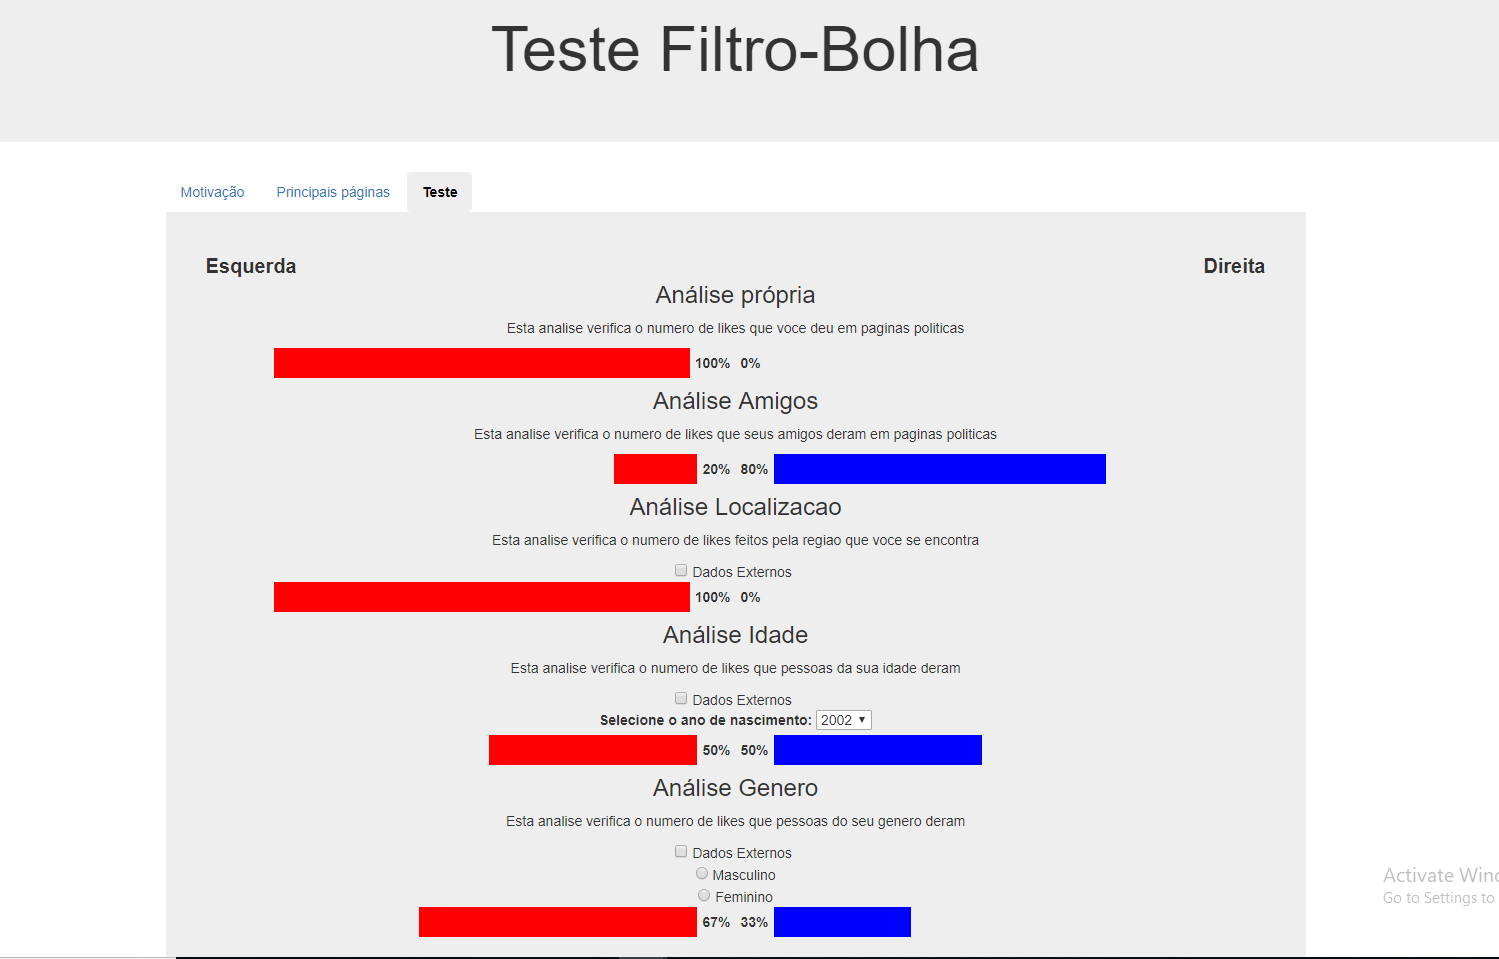
\includegraphics[scale=0.4]{figura1.png}
	\label{fig:figura1}
\end{figure}

\begin{figure}[H]
	\centering
	\caption{Exemplo de chamada REST para a listagem de dados no servidor}
	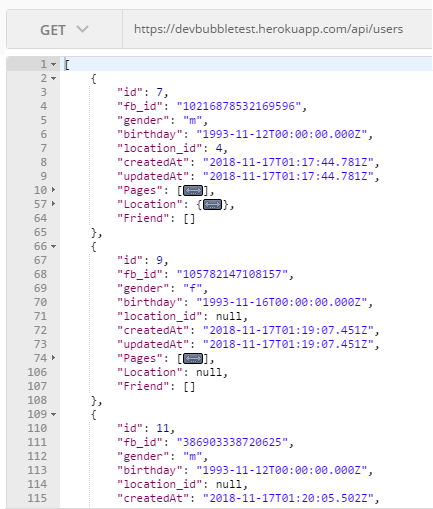
\includegraphics[scale=0.7]{figura2.png}
	\label{fig:figura2}
\end{figure}

Outro ponto a se salientar é o fato de que a avaliação de posicionamento politico das amizades do usuário se refere apenas aos que estão conectados no app. As amizades do usuário que não aprovaram as permissões da aplicação, não aparecem como conexão do usuário. Este é um bloqueio explícito do Facebook na Graph API. Entretando, a análise de dados relacionada à localização e gênero independem da conexão ou não com o usuário. Como todo usuário é adicionado a base de dados do projeto quando entra na aplicação, tem-se as informações demográficas e geográficas persistidas no banco. O modelo de banco utilizado é o descrito na imagem \ref{img:bancoDeDados}.

Além da visualização relacionadas ao perfil do usuário, há também a possibilidade de se comparar os dados apresentados pela aplicação com dados externos, de fora da aplicação do Facebook. Cada estado possui os dados da última eleição (segundo turno), fornecidos pelo TSE (Adicionar SIGLA) e os dados sobre a última pesquisa de opinião realizada pelo Instituto DataFolha (REFERENCIA AQUI), já que o TSE não disponibiliza dados sobre o gênero, localidade e idade de quem votou. 

Quanto aos dados demográficos e geográficos armazenados, todos podem ser acessados pela API localizada no mesmo endereço da aplicação. No anexo \ref{anexoC} é possivel ver todos as chamadas possiveis dentro da API, juntamente com os resultados esperados. 

\chapter{Discussão}

Tirando-se as dificuldades de desenvolvimento, que impediram a aplicação de ser lançada publicamente, não apenas para usuários pré-aprovados, inferir conclusões através dos dados seria extremamente difícil. Inicialmente, o plano do projeto era uma ampla divulgação em páginas de temáticas políticas, para que se tivesse uma amostra bem grande, e uma divulgação ampla em páginas dos dois lados do espectro político da esfera pública. Porém, mesmo desta forma, fica difícil garantir uma amostra sem viés. 

Quanto a análise do usuário, a análise por amizades e páginas curtidas é eficaz pois considera quem cria conteúdos e quem potencialmente os compartilha. Porém, o universo de amigos se restringe apenas aos presentes na aplicação, e também se desconsidera totalmente o algorítimo que fornece o conteúdo ao usuário, feito pelo Facebook. Alguns testes realizados mostram que após um tempo elevado de conexão no Facebook, muitas vezes é trazido um conteúdo pouco comum ao usuário, já que o tempo elevado na aplicação o fez percorrer por todas as temáticas que já lhe são familiares. Existem outros fatores, como engajamento em postagens de amigos por meio de comentários, que fazem também com que o Facebook considere que aquele conteúdo é algo que te interessa e que vale a pena lhe trazer novamente. Há também o fator de \textit{marketing} pago, que a aplicação do projeto não cobre. Uma melhor análise poderia ser feita se fosse possível uma análise do conteúdo trazido pelo Facebook diretamente. Tal funcionalidade existe na Graph API, porém nos últimos anos foi restringida a fabricantes de aplicativos nativos do Facebook, como empresas de telefonia. No \ref{anexoB} é possível ver uma das diversas tentativas de contato com a equipe de desenvolvimento do projeto, explicando o porquê seria interessante a liberação desta permissão para a aplicação. Não foi obtido sucesso na requisição.

Outro ponto que foi tratado durante o desenvolvimento do projeto foi a implementação da autenticação por \textit{token}, ou \textit{OAuth}. Este tipo de autenticação com o servidor foi por um tempo pré-requisito do Facebook, mas posteriormente esse requisito foi retirado. A preocupação do Facebook era que o \textit{id} do usuário fornecido pela Graph API, apesar de diferente entre as aplicações, era possivel acessar o perfil da pessoa diretamente, colocando este \textit{id} na \textit{url}. Porém, uma atualização recente da Graph API fez com que o \textit{id} não seja mais o localizador do perfil quando inserido diretamente na \textit{url}.

\chapter{Conclusão}

Este \textit{template} apresenta as regras básicas para a elaboração do trabalho segundo as normas ABNT.


Além das regras básicas previstas aqui, solicita-se consultar outros detalhes da norma ABNT sempre que se desejar inserir ou configurar algum elemento não previsto aqui. Ou seja, mesmo que este \textit{template} não preveja as demais regras ABNT, por ser uma visão simplificada, ainda assim elas precisam ser seguidas. O anexo \ref{anexoA} deste documento apresenta um resumo das normas ABNT, mas ainda assim também não completo.

Texto de exemplo, texto de exemplo, texto de exemplo, texto de exemplo, texto de exemplo, texto de exemplo, texto de exemplo, texto de exemplo, texto de exemplo, texto de exemplo, texto de exemplo, texto de exemplo, texto de exemplo, texto de exemplo, texto de exemplo, texto de exemplo, texto de exemplo, texto de exemplo, texto de exemplo, texto de exemplo, texto de exemplo, texto de exemplo.  

A tabela \ref{tab:ExemploDeTabela1} é um exemplo de como apresentar tabelas de acordo com essa norma. Veja mais detalhes no anexo \ref{anexoA} deste documento.

%-------------------------------------------------------------------------
% Informações sobre ``tabela''
% 
% Caption(Título) de tabelas e ilustração (tais como figura, gráfico, 
% algoritmo, fotografia, quadro, etc.) sempre acima da própria.
%
% Para todos os captions/(títulos) (de seções, subseções, tabelas, 
% ilustrações, etc):
%     - em maiúscula apenas a primeira letra da sentença (do título), 
%       exceto nomes próprios, geográficos, institucionais ou Programas ou
%       Projetos ou siglas, os quais podem ter letras em maiúscula também.
%
% Todas  as tabelas, ilustrações (figuras, quadros, gráficos, etc. ), 
% anexos, apêndices devem obrigatoriamente ser citados no texto.
%      - a citação deve vir sempre antes da primeira vez em que a tabela, 
%        ilustração, etc., aparecer pela primeira vez.
%
% Não confundir ``tabela'' com ``quadro''. Uma tabela deve ter dados 
% numéricos como informação central. Outros tipos de organização de 
% informações devem ser apresentados em quadros, que é um dos tipos de 
% ilustração. A formatação de um quadro é muito parecida a de uma tabela, 
% porém todos os traços horizontais e verticais devem ser apresentados.
%
%-------------------------------------------------------------------------
\begin{table}[htbp]
	\centering
	\caption{Exemplo de título de tabela}
		\begin{tabular}{p{1in} p{1in} p{1in} p{1in} } \hline

		Cabeçalho 1	& Cabeçalho 2	& Cabeçalho 3	& Cabeçalho 4 \\ \hline
		Texto	& número & número	& número \\ 
		Texto	& número & número	& número \\ 
		Texto	& número & número	& número \\ 
		Texto	& número & número	& número \\ 
		Texto	& número & número	& número \\ \hline
		
		\end{tabular}
	\label{tab:ExemploDeTabela1}
  \source{Marcelo Fantinato, 2015}
\end{table}

Texto de exemplo, texto de exemplo, texto de exemplo, texto de exemplo, texto de exemplo, texto de exemplo, texto de exemplo, texto de exemplo, texto de exemplo, texto de exemplo, texto de exemplo, texto de exemplo, texto de exemplo, texto de exemplo, texto de exemplo, texto de exemplo, texto de exemplo, texto de exemplo, texto de exemplo, texto de exemplo, texto de exemplo, texto de exemplo.

A seguir é apresentado um exemplo de lista de marcadores de apenas um nível (se você finalizar cada item da lista com ponto e vírgula, elas devem ser iniciadas com letra minúsculas; se você finalizar cada item da lista com ponto, elas devem ser iniciadas com letra maiúsculas):
\begin{itemize}
	\item sentença A;
	\item sentença B mais texto mais texto mais texto mais texto mais texto mais texto mais texto mais texto mais texto mais texto mais texto mais texto mais texto mais texto mais texto mais texto mais texto mais texto mais texto mais texto mais texto mais texto mais texto mais texto mais texto;
	\item sentença C;
	\item sentença D mais texto mais texto mais texto mais texto mais texto mais texto mais texto mais texto mais texto mais texto mais texto mais texto mais texto.
\end{itemize}

A seguir é apresentado um exemplo de lista de numeração de apenas um nível (se você finalizar cada item da lista com ponto e vírgula, elas devem ser iniciadas com letra minúsculas; se você finalizar cada item da lista com ponto, elas devem ser iniciadas com letra maiúsculas):
\begin{enumerate}
	\item Sentença A.
	\item Sentença B mais texto mais texto mais texto mais texto mais texto mais texto mais texto mais texto mais texto mais texto mais texto mais texto mais texto mais texto mais texto mais texto mais texto mais texto mais texto mais texto mais texto mais texto mais texto mais texto mais texto.
	\item Sentença C.
	\item Sentença D mais texto mais texto mais texto mais texto mais texto mais texto mais texto mais texto mais texto mais texto mais texto mais texto mais texto.
	\item Sentença E.
	\item Sentença F.
\end{enumerate}

A seguir é apresentado um exemplo de lista de marcadores vários níveis (se você finalizar cada item da lista com ponto e vírgula, elas devem ser iniciadas com letra minúsculas; se você finalizar cada item da lista com ponto, elas devem ser iniciadas com letra maiúsculas):
\begin{itemize}
	\item sentença A:
  \begin{itemize}
	   \item sentença A.1;
	   \item sentença A.2:
     \begin{itemize}
	      \item sentença A.2.1;
	      \item sentença A.2.2;
	      \item sentença A.2.3.
     \end{itemize}
	   \item sentença A.3.
  \end{itemize}
	\item sentença B:
  \begin{itemize}
	   \item sentença B.1:
     \begin{itemize}
	      \item sentença B.1.1;
	      \item sentença B.1.2;
	      \item sentença B.1.3.
     \end{itemize}
	   \item sentença B.2;
	   \item sentença B.3.
  \end{itemize}
\end{itemize}

A seguir é apresentado um exemplo de lista de numeração de vários níveis (se você finalizar cada item da lista com ponto e vírgula, elas devem ser iniciadas com letra minúsculas; se você finalizar cada item da lista com ponto, elas devem ser iniciadas com letra maiúsculas):

\begin{enumerate}
	\item Sentença A:
  \begin{enumerate}
	  \item Sentença A.1.
	  \item Sentença A.2:
    \begin{enumerate}
	    \item Sentença A.2.1.
	    \item Sentença A.2.2.
	    \item Sentença A.2.3.
    \end{enumerate}
	  \item Sentença A.3.
	\end{enumerate}
  \item Sentença B:
  \begin{enumerate}
	  \item Sentença B.1:
      \begin{enumerate}
  	    \item Sentença B.1.1.
  	    \item Sentença B.1.2.
  	    \item Sentença B.1.3.
      \end{enumerate}
	  \item Sentença B.2.
	  \item Sentença B.3.
  \end{enumerate}
\end{enumerate}

A figura \ref{fig:figura-exemplo1} é um exemplo de como apresentar ilustrações de acordo com essa norma. Qualquer outra ilustração deve ser apresentada de forma similar, mudando apenas o prefixo do título e a numeração. Veja mais detalhes no anexo \ref{anexoA} deste documento.

%-------------------------------------------------------------------------
% Informações sobre ``figura''
% 
% Caption(Título) de tabelas e ilustração (tais como figura, gráfico, 
% algoritmo, fotografia, quadro, etc.) sempre acima da própria.
%
% Para todos os captions/(títulos) (de seções, subseções, tabelas, 
% ilustrações, etc):
%     - em maiúscula apenas a primeira letra da sentença (do título), 
%       exceto nomes próprios, geográficos, institucionais ou Programas ou
%       Projetos ou siglas, os quais podem ter letras em maiúscula também.
%
% Fonte de ilustração (tais como figura, gráfico, algoritmo, fotografia, 
% quadro, etc.) sempre abaixo da própria.
%      - se a fonte for o próprio autor, colocar o nome dele. 
%      - se a fonte for outro autor, citar sua referência.
%
% Todas  as tabelas, ilustrações (figuras, quadros, gráficos, etc. ), 
% anexos, apêndices devem obrigatoriamente ser citados no texto.
%      - a citação deve vir sempre antes da primeira vez em que a tabela, 
%        ilustração, etc., aparecer pela primeira vez.
%
%-------------------------------------------------------------------------
\begin{figure}[H]% H manda colocar exatamente nessa posição no texto (relativa aos parágrafos anterior e posterior)
	\centering
 	  \caption{Exemplo de título de ilustração do tipo figura}
		
\includegraphics{figura-exemplo.png}
	\label{fig:figura-exemplo1}
  \source{Marcelo Fantinato, 2015}
\end{figure}

Texto de exemplo, texto de exemplo, texto de exemplo, texto de exemplo, texto de exemplo, texto de exemplo, texto de exemplo, texto de exemplo, texto de exemplo, texto de exemplo, texto de exemplo, texto de exemplo, texto de exemplo, texto de exemplo, texto de exemplo, texto de exemplo, texto de exemplo, texto de exemplo, texto de exemplo, texto de exemplo, texto de exemplo, texto de exemplo.

\section{Uma seção secundária}
 
Texto de exemplo, texto de exemplo, texto de exemplo, texto de exemplo, texto de exemplo, texto de exemplo, texto de exemplo, texto de exemplo, texto de exemplo, texto de exemplo, texto de exemplo, texto de exemplo, texto de exemplo, texto de exemplo, texto de exemplo, texto de exemplo, texto de exemplo, texto de exemplo, texto de exemplo, texto de exemplo, texto de exemplo, texto de exemplo, texto de exemplo.

A figura \ref{fig:figura-exemplo2} é um exemplo de como apresentar ilustrações de acordo com essa norma. Qualquer outra ilustração deve ser apresentada de forma similar, mudando apenas o prefixo do título e a numeração. Veja mais detalhes no anexo \ref{anexoA} deste documento.

\begin{figure}[htbp]
	\centering
  \caption{Exemplo de título de ilustração do tipo figura, que pode ser maior para apresentar mais explicações sobre o conteúdo da figura, se for o caso}
		
\includegraphics{figura-exemplo.png}
	\label{fig:figura-exemplo2}
  \source{Marcelo Fantinato, 2015}
\end{figure}

Texto de exemplo, texto de exemplo, texto de exemplo, texto de exemplo, texto de exemplo, texto de exemplo, texto de exemplo, texto de exemplo, texto de exemplo, texto de exemplo, texto de exemplo, texto de exemplo, texto de exemplo, texto de exemplo, texto de exemplo, texto de exemplo, texto de exemplo, texto de exemplo, texto de exemplo, texto de exemplo, texto de exemplo, texto de exemplo, texto de exemplo.

\subsection{Uma seção terciária}

Texto de exemplo, texto de exemplo, texto de exemplo, texto de exemplo, texto de exemplo, texto de exemplo, texto de exemplo, texto de exemplo, texto de exemplo, texto de exemplo, texto de exemplo, texto de exemplo, texto de exemplo, texto de exemplo, texto de exemplo, texto de exemplo, texto de exemplo, texto de exemplo, texto de exemplo, texto de exemplo, texto de exemplo, texto de exemplo, texto de exemplo.

A tabela \ref{tab:ExemploDeTabela2} é outro exemplo de como apresentar tabelas de acordo com essa norma. Veja mais detalhes no anexo \ref{anexoA} deste documento.

\begin{table}[htbp]
	\centering
	\caption{Exemplo de título de tabela, que pode ser maior para apresentar mais explicações sobre o conteúdo da tabela, se for o caso}
		\begin{tabular}{p{1.2in} p{1.2in} p{1.2in} p{1.2in} } \hline
		
		Cabeçalho 1	& Cabeçalho 2	& Cabeçalho 3	& Cabeçalho 4 \\ \hline
		Texto	& número & número	& número \\ 
		Texto	& número & número	& número \\ 
		Texto	& número & número	& número \\ 
		Texto	& número & número	& número \\ 
		Texto	& número & número	& número \\ \hline
			
		\end{tabular}
	\label{tab:ExemploDeTabela2}
  \source{Marcelo Fantinato, 2015}
\end{table}

\subsection{Outra seção terciária}

Texto de exemplo, texto de exemplo, texto de exemplo, texto de exemplo, texto de exemplo, texto de exemplo, texto de exemplo, texto de exemplo, texto de exemplo, texto de exemplo, texto de exemplo, texto de exemplo, texto de exemplo, texto de exemplo, texto de exemplo, texto de exemplo, texto de exemplo, texto de exemplo, texto de exemplo, texto de exemplo, texto de exemplo, texto de exemplo, texto de exemplo.

Texto de exemplo, texto de exemplo, texto de exemplo, texto de exemplo, texto de exemplo, texto de exemplo, texto de exemplo, texto de exemplo, texto de exemplo, texto de exemplo, texto de exemplo, texto de exemplo, texto de exemplo, texto de exemplo, texto de exemplo, texto de exemplo, texto de exemplo, texto de exemplo, texto de exemplo, texto de exemplo, texto de exemplo, texto de exemplo, texto de exemplo.

A figura \ref{fig:figura-exemplo3} é um exemplo de como apresentar ilustrações de acordo com essa norma. Qualquer outra ilustração deve ser apresentada de forma similar, mudando apenas o prefixo do título e a numeração. Veja mais detalhes no anexo \ref{anexoA} deste documento.

\begin{figure}[htbp]
	\centering
	\caption{Exemplo de título de ilustração do tipo figura}
		
\includegraphics{figura-exemplo.png}
	\label{fig:figura-exemplo3}
  \source{Marcelo Fantinato, 2015}
\end{figure}

\subsection{Mais uma seção terciária}

Texto de exemplo, texto de exemplo, texto de exemplo, texto de exemplo, texto de exemplo, texto de exemplo, texto de exemplo, texto de exemplo, texto de exemplo, texto de exemplo, texto de exemplo, texto de exemplo, texto de exemplo, texto de exemplo, texto de exemplo, texto de exemplo, texto de exemplo, texto de exemplo, texto de exemplo, texto de exemplo, texto de exemplo, texto de exemplo, texto de exemplo.

A tabela \ref{tab:ExemploDeTabela3} é um exemplo de como apresentar tabelas de acordo com essa norma. Veja mais detalhes no anexo \ref{anexoA} deste documento.

\begin{table}[htbp]
	\centering
	\caption{Exemplo de título de tabela}
		\begin{tabular}{p{0.85in} p{0.85in} p{0.85in} p{0.85in} } \hline
		
		Cabeçalho 1	& Cabeçalho 2	& Cabeçalho 3	& Cabeçalho 4 \\ \hline
		Texto	& número & número	& número \\ 
		Texto	& número & número	& número \\ 
		Texto	& número & número	& número \\ 
		Texto	& número & número	& número \\ 
		Texto	& número & número	& número \\ \hline
			
		\end{tabular}
	\label{tab:ExemploDeTabela3}
  \source{Marcelo Fantinato, 2015}
\end{table}


A figura \ref{fig:figura-exemplo4} é um exemplo de como apresentar ilustrações de acordo com essa norma. Qualquer outra ilustração deve ser apresentada de forma similar, mudando apenas o prefixo do título e a numeração. Veja mais detalhes no anexo \ref{anexoA} deste documento.

\begin{figure}[htbp]
	\centering
	\caption{Exemplo de título bem grande de ilustração do tipo figura, bem grande bem grande bem grande bem grande bem grande bem grande bem grande bem grande bem grande bem grande bem grande bem grande bem grande bem grande bem grande bem grande bem grande bem grande bem grande bem grande bem grande bem grande bem grande bem grande bem grande bem grande bem grande bem grande bem grande bem grande bem grande bem grande}
		
\includegraphics{figura-exemplo.png}
	\label{fig:figura-exemplo4}
  \source{Marcelo Fantinato, 2015}
\end{figure}

Texto de exemplo, texto de exemplo, texto de exemplo, texto de exemplo, texto de exemplo, texto de exemplo, texto de exemplo, texto de exemplo, texto de exemplo, texto de exemplo, texto de exemplo, texto de exemplo, texto de exemplo, texto de exemplo, texto de exemplo, texto de exemplo, texto de exemplo, texto de exemplo, texto de exemplo, texto de exemplo, texto de exemplo, texto de exemplo, texto de exemplo.

\section{Outra seção secundária}

Texto de exemplo, texto de exemplo, texto de exemplo, texto de exemplo, texto de exemplo, texto de exemplo, texto de exemplo, texto de exemplo, texto de exemplo, texto de exemplo, texto de exemplo, texto de exemplo, texto de exemplo, texto de exemplo, texto de exemplo, texto de exemplo, texto de exemplo, texto de exemplo, texto de exemplo, texto de exemplo, texto de exemplo, texto de exemplo, texto de exemplo.

Texto de exemplo, texto de exemplo, texto de exemplo, texto de exemplo, texto de exemplo, texto de exemplo, texto de exemplo, texto de exemplo, texto de exemplo, texto de exemplo, texto de exemplo, texto de exemplo, texto de exemplo, texto de exemplo, texto de exemplo, texto de exemplo, texto de exemplo, texto de exemplo, texto de exemplo, texto de exemplo, texto de exemplo, texto de exemplo, texto de exemplo.

A tabela \ref{tab:ExemploDeTabela4} é outro exemplo de como apresentar tabelas de acordo com essa norma. Veja mais detalhes no anexo \ref{anexoA} deste documento.

\begin{table}[htbp]
	\centering
	\caption{Exemplo de título bem grande de tabela, bem grande bem grande bem grande bem grande bem grande bem grande bem grande bem grande bem grande bem grande bem grande bem grande bem grande bem grande bem grande bem grande bem grande bem grande bem grande bem grande bem grande bem grande bem grande bem grande bem grande bem grande bem grande bem grande bem grande bem grande bem grande bem grande}
		\begin{tabular}{p{1.4in} p{1.4in} p{1.4in} p{1.4in} } \hline
		
		Cabeçalho 1	& Cabeçalho 2	& Cabeçalho 3	& Cabeçalho 4 \\ \hline
		Texto	& número & número	& número \\ 
		Texto	& número & número	& número \\ 
		Texto	& número & número	& número \\ 
		Texto	& número & número	& número \\ 
		Texto	& número & número	& número \\ \hline
			
		\end{tabular}
	\label{tab:ExemploDeTabela4}
  \source{Marcelo Fantinato, 2015}
\end{table}

Texto de exemplo, texto de exemplo, texto de exemplo, texto de exemplo, texto de exemplo, texto de exemplo, texto de exemplo, texto de exemplo, texto de exemplo, texto de exemplo, texto de exemplo, texto de exemplo, texto de exemplo, texto de exemplo, texto de exemplo, texto de exemplo, texto de exemplo, texto de exemplo, texto de exemplo, texto de exemplo, texto de exemplo, texto de exemplo, texto de exemplo.

A tabela \ref{tab:ExemploDeTabela5} é outro exemplo de como apresentar tabelas de acordo com essa norma. Veja mais detalhes no anexo \ref{anexoA} deste documento.

\begin{table}[htbp]
	\centering
	\caption{Exemplo de título de tabela}
		\begin{tabular}{p{1.0in} p{1.0in} p{1.0in} } \hline
		
		Cabeçalho 1	& Cabeçalho 2	& Cabeçalho 3	 \\ \hline
		número & número	& número \\ 
		número & número	& número \\ 
		número & número	& número \\ 
		número & número	& número \\ 
		número & número	& número \\ \hline
			
		\end{tabular}
	\label{tab:ExemploDeTabela5}
  \source{Marcelo Fantinato, 2015}
\end{table}


Texto de exemplo, texto de exemplo, texto de exemplo, texto de exemplo, texto de exemplo, texto de exemplo, texto de exemplo, texto de exemplo, texto de exemplo, texto de exemplo, texto de exemplo, texto de exemplo, texto de exemplo, texto de exemplo, texto de exemplo, texto de exemplo, texto de exemplo, texto de exemplo, texto de exemplo, texto de exemplo, texto de exemplo, texto de exemplo, texto de exemplo.

\section{Mais uma seção secundária}

Texto de exemplo, texto de exemplo, texto de exemplo, texto de exemplo, texto de exemplo, texto de exemplo, texto de exemplo, texto de exemplo, texto de exemplo, texto de exemplo, texto de exemplo, texto de exemplo, texto de exemplo, texto de exemplo, texto de exemplo, texto de exemplo, texto de exemplo, texto de exemplo, texto de exemplo, texto de exemplo, texto de exemplo, texto de exemplo, texto de exemplo.

A figura \ref{fig:figura-exemplo5} é um exemplo de como apresentar ilustrações de acordo com essa norma. Qualquer outra ilustração deve ser apresentada de forma similar, mudando apenas o prefixo do título e a numeração. Veja mais detalhes no anexo \ref{anexoA} deste documento.

\begin{figure}[htbp]
	\centering
	\caption{Exemplo de título de ilustração do tipo figura}
		
\includegraphics{figura-exemplo.png}
	\label{fig:figura-exemplo5}
  \source{Marcelo Fantinato, 2015}
\end{figure}

Texto de exemplo, texto de exemplo, texto de exemplo, texto de exemplo, texto de exemplo, texto de exemplo, texto de exemplo, texto de exemplo, texto de exemplo, texto de exemplo, texto de exemplo, texto de exemplo, texto de exemplo, texto de exemplo, texto de exemplo, texto de exemplo, texto de exemplo, texto de exemplo.

\chapter{Outra seção primária}

Texto de exemplo, texto de exemplo, texto de exemplo, texto de exemplo, texto de exemplo, texto de exemplo, texto de exemplo, texto de exemplo, texto de exemplo, texto de exemplo, texto de exemplo, texto de exemplo, texto de exemplo, texto de exemplo, texto de exemplo, texto de exemplo, texto de exemplo, texto de exemplo, texto de exemplo, texto de exemplo, texto de exemplo, texto de exemplo, texto de exemplo.

Lembrar de fazer as devidas \citeonline{teste1} referências, tal como \cite{teste1, teste2, teste3}.

O algoritmo \ref{alg:algoritmo-exemplo1} é um exemplo de como apresentar ilustrações de acordo com essa norma. Qualquer outra ilustração deve ser apresentada de forma similar, mudando apenas o prefixo do título e a numeração. Veja mais detalhes no anexo \ref{anexoA} deste documento.

%-------------------------------------------------------------------------
% Informações sobre ``algoritmo''
% 
% Caption(Título) de tabelas e ilustração (tais como figura, gráfico, 
% algoritmo, fotografia, quadro, etc.) sempre acima da própria.
%
% Para todos os captions/(títulos) (de seções, subseções, tabelas, 
% ilustrações, etc):
%     - em maiúscula apenas a primeira letra da sentença (do título), 
%       exceto nomes próprios, geográficos, institucionais ou Programas ou
%       Projetos ou siglas, os quais podem ter letras em maiúscula também.
%
% Fonte de ilustração (tais como figura, gráfico, algoritmo, fotografia, 
% quadro, etc.) sempre abaixo da própria.
%      - se a fonte for o próprio autor, colocar o nome dele. 
%      - se a fonte for outro autor, citar sua referência.
%
% Todas  as tabelas, ilustrações (figuras, quadros, gráficos, etc. ), 
% anexos, apêndices devem obrigatoriamente ser citados no texto.
%      - a citação deve vir sempre antes da primeira vez em que a tabela, 
%        ilustração, etc., aparecer pela primeira vez.
%
%-------------------------------------------------------------------------
\begin{algorithm}[htbp]
\caption{Exemplo de título de ilustração do tipo algoritmo, que pode ser maior para apresentar mais explicações sobre o conteúdo do algoritmo, se for o caso}
\label{alg:algoritmo-exemplo1}
\begin{algorithmic}[1]
\Procedure{MyProcedure}{}
\State $passo-1$
\State $passo-2$
\State $passo-3$
\State $.$
\State $.$
\State $.$
\State $.$
\State $.$
\State $passo-n$
\EndProcedure
\end{algorithmic}
\source{Marcelo Fantinato, 2015}
\end{algorithm}


Texto de exemplo, texto de exemplo, texto de exemplo, texto de exemplo, texto de exemplo, texto de exemplo, texto de exemplo, texto de exemplo, texto de exemplo, texto de exemplo, texto de exemplo, texto de exemplo, texto de exemplo, texto de exemplo, texto de exemplo, texto de exemplo, texto de exemplo, texto de exemplo, texto de exemplo, texto de exemplo, texto de exemplo, texto de exemplo.

\section{Uma seção secundária}

Texto de exemplo, texto de exemplo, texto de exemplo, texto de exemplo, texto de exemplo, texto de exemplo, texto de exemplo, texto de exemplo, texto de exemplo, texto de exemplo, texto de exemplo, texto de exemplo, texto de exemplo, texto de exemplo, texto de exemplo, texto de exemplo, texto de exemplo, texto de exemplo, texto de exemplo, texto de exemplo, texto de exemplo, texto de exemplo, texto de exemplo.

As fórmulas \ref{eq:equacao-exemplo1} e \ref{eq:equacao-exemplo2} são exemplos de como apresentar fórmulas e equações destacadas do parágrafo normal do texto. Veja mais detalhes no anexo \ref{anexoA} deste documento.

\begin{equation}
  X + Y = Z
	\label{eq:equacao-exemplo1}
\end{equation}

\begin{equation}
  (X - Y)/5 = n
	\label{eq:equacao-exemplo2}
\end{equation}


O algoritmo \ref{alg:algoritmo-exemplo2} é um exemplo de como apresentar ilustrações de acordo com essa norma. Qualquer outra ilustração deve ser apresentada de forma similar, mudando apenas o prefixo do título e a numeração. Veja mais detalhes no anexo \ref{anexoA} deste documento.

\begin{algorithm}[htbp]
\caption{Exemplo de título de ilustração do tipo algoritmo}
\label{alg:algoritmo-exemplo2}
\begin{algorithmic}[1]
\Procedure{MyProcedure}{}
\State $passo-1$
\State $passo-2$
\State $passo-3$
\State $.$
\State $.$
\State $.$
\State $.$
\State $.$
\State $passo-n$
\EndProcedure
\end{algorithmic}
\source{Marcelo Fantinato, 2015}
\end{algorithm}

Texto de exemplo, texto de exemplo, texto de exemplo, texto de exemplo, texto de texto de exemplo, texto de exemplo, texto de exemplo, texto de exemplo, texto de exemplo, texto de exemplo, texto de exemplo, texto de exemplo, texto de exemplo, texto de exemplo, texto de exemplo, texto de exemplo, texto de exemplo, texto de exemplo, texto de exemplo, texto de exemplo, texto de exemplo, texto de exemplo.

\subsection{Uma seção terciária}

Texto de exemplo, texto de exemplo, texto de exemplo, texto de exemplo, texto de exemplo, texto de exemplo, texto de exemplo, texto de exemplo, texto de exemplo, texto de exemplo, texto de exemplo, texto de exemplo, texto de exemplo, texto de exemplo, texto de exemplo, texto de exemplo, texto de exemplo, texto de exemplo, texto de exemplo, texto de exemplo, texto de exemplo, texto de exemplo, texto de exemplo.

O algoritmo \ref{alg:algoritmo-exemplo3} é um exemplo de como apresentar ilustrações de acordo com essa norma. Qualquer outra ilustração deve ser apresentada de forma similar, mudando apenas o prefixo do título e a numeração. Veja mais detalhes no anexo \ref{anexoA} deste documento.

\begin{algorithm}[htbp]
\caption{Exemplo de título de ilustração do tipo algoritmo}
\label{alg:algoritmo-exemplo3}
\begin{algorithmic}[1]
\Procedure{MyProcedure}{}
\State $passo-1$
\State $passo-2$
\State $passo-3$
\State $.$
\State $.$
\State $.$
\State $.$
\State $.$
\State $passo-n$
\EndProcedure
\end{algorithmic}
\source{Marcelo Fantinato, 2015}
\end{algorithm}


\subsection{Outra seção terciária}

Texto de exemplo, texto de exemplo, texto de exemplo, texto de exemplo, texto de exemplo, texto de exemplo, texto de exemplo, texto de exemplo, texto de exemplo, texto de exemplo, texto de exemplo, texto de exemplo, texto de exemplo, texto de exemplo, texto de exemplo, texto de exemplo, texto de exemplo, texto de exemplo, texto de exemplo, texto de exemplo, texto de exemplo, texto de exemplo, texto de exemplo.

\subsection{Mais uma seção terciária}

Texto de exemplo, texto de exemplo, texto de exemplo, texto de exemplo, texto de exemplo, texto de exemplo, texto de exemplo, texto de exemplo, texto de exemplo, texto de exemplo, texto de exemplo, texto de exemplo, texto de exemplo, texto de exemplo, texto de exemplo, texto de exemplo, texto de exemplo, texto de exemplo, texto de exemplo, texto de exemplo, texto de exemplo, texto de exemplo, texto de exemplo.

Texto de exemplo, texto de exemplo, texto de exemplo, texto de exemplo, texto de exemplo, texto de exemplo, texto de exemplo, texto de exemplo, texto de exemplo, texto de exemplo, texto de exemplo, texto de exemplo, texto de exemplo, texto de exemplo, texto de exemplo, texto de exemplo, texto de exemplo, texto de exemplo, texto de exemplo, texto de exemplo, texto de exemplo, texto de exemplo, texto de exemplo.

O algoritmo \ref{alg:algoritmo-exemplo4} é um exemplo de como apresentar ilustrações de acordo com essa norma. Qualquer outra ilustração deve ser apresentada de forma similar, mudando apenas o prefixo do título e a numeração. Veja mais detalhes no anexo \ref{anexoA} deste documento.

\begin{algorithm}[htbp]
\caption{Exemplo de título bem grande de ilustração do tipo algoritmo, bem grande bem grande bem grande bem grande bem grande bem grande bem grande bem grande bem grande bem grande bem grande bem grande bem grande bem grande bem grande bem grande bem grande bem grande bem grande bem grande bem grande bem grande bem grande bem grande bem grande bem grande bem grande bem grande bem grande bem grande}
\label{alg:algoritmo-exemplo4}
\begin{algorithmic}[1]
\Procedure{MyProcedure}{}
\State $passo-1$
\State $passo-2$
\State $passo-3$
\State $.$
\State $.$
\State $.$
\State $.$
\State $.$
\State $passo-n$
\EndProcedure
\end{algorithmic}
\source{Marcelo Fantinato, 2015}
\end{algorithm}


Texto de exemplo, texto de exemplo, texto de exemplo, texto de exemplo, texto de texto de exemplo, texto de exemplo, texto de exemplo, texto de exemplo, texto de exemplo, texto de exemplo, texto de exemplo, texto de exemplo, texto de exemplo, texto de exemplo, texto de exemplo, texto de exemplo, texto de exemplo, texto de exemplo, texto de exemplo, texto de exemplo, texto de exemplo, texto de exemplo.

\section{Outra seção secundária}

Texto de exemplo, texto de exemplo, texto de exemplo, texto de exemplo, texto de exemplo, texto de exemplo, texto de exemplo, texto de exemplo, texto de exemplo, texto de exemplo, texto de exemplo, texto de exemplo, texto de exemplo, texto de exemplo, texto de exemplo, texto de exemplo, texto de exemplo, texto de exemplo, texto de exemplo, texto de exemplo, texto de exemplo, texto de exemplo, texto de exemplo.

Texto de exemplo, texto de exemplo, texto de exemplo, texto de exemplo, texto de exemplo, texto de exemplo, texto de exemplo, texto de exemplo, texto de exemplo, texto de exemplo, texto de exemplo, texto de exemplo, texto de exemplo, texto de exemplo, texto de exemplo, texto de exemplo, texto de exemplo, texto de exemplo, texto de exemplo, texto de exemplo, texto de exemplo, texto de exemplo, texto de exemplo.

Texto de exemplo, texto de exemplo, texto de exemplo, texto de exemplo, texto de exemplo, texto de exemplo, texto de exemplo, texto de exemplo, texto de exemplo, texto de exemplo, texto de exemplo, texto de exemplo, texto de exemplo, texto de exemplo, texto de exemplo, texto de exemplo, texto de exemplo, texto de exemplo, texto de exemplo, texto de exemplo, texto de exemplo, texto de exemplo, texto de exemplo.

\section{Mais uma seção secundária}

Texto de exemplo, texto de exemplo, texto de exemplo, texto de exemplo, texto de exemplo, texto de exemplo, texto de exemplo, texto de exemplo, texto de exemplo, texto de exemplo, texto de exemplo, texto de exemplo, texto de exemplo, texto de exemplo, texto de exemplo, texto de exemplo, texto de exemplo, texto de exemplo, texto de exemplo, texto de exemplo, texto de exemplo, texto de exemplo, texto de exemplo.

Texto de exemplo, texto de exemplo, texto de exemplo, texto de exemplo, texto de exemplo, texto de exemplo, texto de exemplo, texto de exemplo, texto de exemplo, texto de exemplo, texto de exemplo, texto de exemplo, texto de exemplo, texto de exemplo, texto de exemplo, texto de exemplo, texto de exemplo, texto de exemplo, texto de exemplo, texto de exemplo, texto de exemplo, texto de exemplo, texto de exemplo.

\chapter{Mais uma seção primária}

Texto de exemplo, texto de exemplo, texto de exemplo, texto de exemplo, texto de exemplo, texto de exemplo, texto de exemplo, texto de exemplo, texto de exemplo, texto de exemplo, texto de exemplo, texto de exemplo, texto de exemplo, texto de exemplo, texto de exemplo, texto de exemplo, texto de exemplo, texto de exemplo, texto de exemplo, texto de exemplo, texto de exemplo, texto de exemplo, texto de exemplo.

Texto de exemplo, texto de exemplo, texto de exemplo, texto de exemplo, texto de exemplo, texto de exemplo, texto de exemplo, texto de exemplo, texto de exemplo, texto de exemplo, texto de exemplo, texto de exemplo, texto de exemplo, texto de exemplo, texto de exemplo, texto de exemplo, texto de exemplo, texto de exemplo, texto de exemplo, texto de exemplo, texto de exemplo, texto de exemplo.

\section{Uma seção secundária}

Texto de exemplo, texto de exemplo, texto de exemplo, texto de exemplo, texto de exemplo, texto de exemplo, texto de exemplo, texto de exemplo, texto de exemplo, texto de exemplo, texto de exemplo, texto de exemplo, texto de exemplo, texto de exemplo, texto de exemplo, texto de exemplo, texto de exemplo, texto de exemplo, texto de exemplo, texto de exemplo, texto de exemplo, texto de exemplo, texto de exemplo.

Texto de exemplo, texto de exemplo, texto de exemplo, texto de exemplo, texto de exemplo, texto de exemplo, texto de exemplo, texto de exemplo, texto de exemplo, texto de exemplo, texto de exemplo, texto de exemplo, texto de exemplo, texto de exemplo, texto de exemplo, texto de exemplo, texto de exemplo, texto de exemplo, texto de exemplo, texto de exemplo, texto de exemplo, texto de exemplo, texto de exemplo.

\subsection{Uma seção terciária}

Texto de exemplo, texto de exemplo, texto de exemplo, texto de exemplo, texto de exemplo, texto de exemplo, texto de exemplo, texto de exemplo, texto de exemplo, texto de exemplo, texto de exemplo, texto de exemplo, texto de exemplo, texto de exemplo, texto de exemplo, texto de exemplo, texto de exemplo, texto de exemplo, texto de exemplo, texto de exemplo, texto de exemplo, texto de exemplo, texto de exemplo.

\subsubsection{Uma seção quartenária}

Texto de exemplo, texto de exemplo, texto de exemplo, texto de exemplo, texto de exemplo, texto de exemplo, texto de exemplo, texto de exemplo, texto de exemplo, texto de exemplo, texto de exemplo, texto de exemplo, texto de exemplo, texto de exemplo, texto de exemplo, texto de exemplo, texto de exemplo, texto de exemplo, texto de exemplo, texto de exemplo, texto de exemplo, texto de exemplo, texto de exemplo.

\subsubsubsection{Uma seção quinária}

Texto de exemplo, texto de exemplo, texto de exemplo, texto de exemplo, texto de exemplo, texto de exemplo, texto de exemplo, texto de exemplo, texto de exemplo, texto de exemplo, texto de exemplo, texto de exemplo, texto de exemplo, texto de exemplo, texto de exemplo, texto de exemplo, texto de exemplo, texto de exemplo, texto de exemplo, texto de exemplo, texto de exemplo, texto de exemplo, texto de exemplo.

\subsubsubsection{Outra seção quinária}

Texto de exemplo, texto de exemplo, texto de exemplo, texto de exemplo, texto de exemplo, texto de exemplo, texto de exemplo, texto de exemplo, texto de exemplo, texto de exemplo, texto de exemplo, texto de exemplo, texto de exemplo, texto de exemplo, texto de exemplo, texto de exemplo, texto de exemplo, texto de exemplo, texto de exemplo, texto de exemplo, texto de exemplo, texto de exemplo, texto de exemplo.

\subsubsubsection{Mais uma seção quinária}

Texto de exemplo, texto de exemplo, texto de exemplo, texto de exemplo, texto de exemplo, texto de exemplo, texto de exemplo, texto de exemplo, texto de exemplo, texto de exemplo, texto de exemplo, texto de exemplo, texto de exemplo, texto de exemplo, texto de exemplo, texto de exemplo, texto de exemplo, texto de exemplo, texto de exemplo, texto de exemplo, texto de exemplo, texto de exemplo, texto de exemplo.

\subsubsection{Outra seção quartenária}

Texto de exemplo, texto de exemplo, texto de exemplo, texto de exemplo, texto de exemplo, texto de exemplo, texto de exemplo, texto de exemplo, texto de exemplo, texto de exemplo, texto de exemplo, texto de exemplo, texto de exemplo, texto de exemplo, texto de exemplo, texto de exemplo, texto de exemplo, texto de exemplo, texto de exemplo, texto de exemplo, texto de exemplo, texto de exemplo, texto de exemplo.

\subsubsection{Mais uma seção quartenária}

Texto de exemplo, texto de exemplo, texto de exemplo, texto de exemplo, texto de exemplo, texto de exemplo, texto de exemplo, texto de exemplo, texto de exemplo, texto de exemplo, texto de exemplo, texto de exemplo, texto de exemplo, texto de exemplo, texto de exemplo, texto de exemplo, texto de exemplo, texto de exemplo, texto de exemplo, texto de exemplo, texto de exemplo, texto de exemplo, texto de exemplo.

\subsection{Outra seção terciária}

Texto de exemplo, texto de exemplo, texto de exemplo, texto de exemplo, texto de exemplo, texto de exemplo, texto de exemplo, texto de exemplo, texto de exemplo, texto de exemplo, texto de exemplo, texto de exemplo, texto de exemplo, texto de exemplo, texto de exemplo, texto de exemplo, texto de exemplo, texto de exemplo, texto de exemplo, texto de exemplo, texto de exemplo, texto de exemplo, texto de exemplo.

\subsection{Mais uma seção terciária}

Texto de exemplo, texto de exemplo, texto de exemplo, texto de exemplo, texto de exemplo, texto de exemplo, texto de exemplo, texto de exemplo, texto de exemplo, texto de exemplo, texto de exemplo, texto de exemplo, texto de exemplo, texto de exemplo, texto de exemplo, texto de exemplo, texto de exemplo, texto de exemplo, texto de exemplo, texto de exemplo, texto de exemplo, texto de exemplo, texto de exemplo.

Texto de exemplo, texto de exemplo, texto de exemplo, texto de exemplo, texto de exemplo, texto de exemplo, texto de exemplo, texto de exemplo, texto de exemplo, texto de exemplo, texto de exemplo, texto de exemplo, texto de exemplo, texto de exemplo, texto de exemplo, texto de exemplo, texto de exemplo, texto de exemplo, texto de exemplo, texto de exemplo, texto de exemplo, texto de exemplo, texto de exemplo.

\section{Outra seção secundária}

Texto de exemplo, texto de exemplo, texto de exemplo, texto de exemplo, texto de exemplo, texto de exemplo, texto de exemplo, texto de exemplo, texto de exemplo, texto de exemplo, texto de exemplo, texto de exemplo, texto de exemplo, texto de exemplo, texto de exemplo, texto de exemplo, texto de exemplo, texto de exemplo, texto de exemplo, texto de exemplo, texto de exemplo, texto de exemplo, texto de exemplo.

Texto de exemplo, texto de exemplo, texto de exemplo, texto de exemplo, texto de exemplo, texto de exemplo, texto de exemplo, texto de exemplo, texto de exemplo, texto de exemplo, texto de exemplo, texto de exemplo, texto de exemplo, texto de exemplo, texto de exemplo, texto de exemplo, texto de exemplo, texto de exemplo, texto de exemplo, texto de exemplo, texto de exemplo, texto de exemplo, texto de exemplo.

Texto de exemplo, texto de exemplo, texto de exemplo, texto de exemplo, texto de exemplo, texto de exemplo, texto de exemplo, texto de exemplo, texto de exemplo, texto de exemplo, texto de exemplo, texto de exemplo, texto de exemplo, texto de exemplo, texto de exemplo, texto de exemplo, texto de exemplo, texto de exemplo, texto de exemplo, texto de exemplo, texto de exemplo, texto de exemplo, texto de exemplo.

\section{Mais uma seção secundária}

Texto de exemplo, texto de exemplo, texto de exemplo, texto de exemplo, texto de exemplo, texto de exemplo, texto de exemplo, texto de exemplo, texto de exemplo, texto de exemplo, texto de exemplo, texto de exemplo, texto de exemplo, texto de exemplo, texto de exemplo, texto de exemplo, texto de exemplo, texto de exemplo, texto de exemplo, texto de exemplo, texto de exemplo, texto de exemplo, texto de exemplo.

Texto de exemplo, texto de exemplo, texto de exemplo, texto de exemplo, texto de exemplo, texto de exemplo, texto de exemplo, texto de exemplo, texto de exemplo, texto de exemplo, texto de exemplo, texto de exemplo, texto de exemplo, texto de exemplo, texto de exemplo, texto de exemplo, texto de exemplo, texto de exemplo, texto de exemplo, texto de exemplo, texto de exemplo, texto de exemplo, texto de exemplo.

\chapter{Mais uma outra seção primária}

Texto de exemplo, texto de exemplo, texto de exemplo, texto de exemplo, texto de exemplo, texto de exemplo, texto de exemplo, texto de exemplo, texto de exemplo, texto de exemplo, texto de exemplo, texto de exemplo, texto de exemplo, texto de exemplo, texto de exemplo, texto de exemplo, texto de exemplo, texto de exemplo, texto de exemplo, texto de exemplo, texto de exemplo, texto de exemplo, texto de exemplo.

Texto de exemplo, texto de exemplo, texto de exemplo, texto de exemplo, texto de exemplo, texto de exemplo, texto de exemplo, texto de exemplo, texto de exemplo, texto de exemplo, texto de exemplo, texto de exemplo, texto de exemplo, texto de exemplo, texto de exemplo, texto de exemplo, texto de exemplo, texto de exemplo, texto de exemplo, texto de exemplo, texto de exemplo, texto de exemplo.

\section{Uma seção secundária}

Texto de exemplo, texto de exemplo, texto de exemplo, texto de exemplo, texto de exemplo, texto de exemplo, texto de exemplo, texto de exemplo, texto de exemplo, texto de exemplo, texto de exemplo, texto de exemplo, texto de exemplo, texto de exemplo, texto de exemplo, texto de exemplo, texto de exemplo, texto de exemplo, texto de exemplo, texto de exemplo, texto de exemplo, texto de exemplo, texto de exemplo.

Texto de exemplo, texto de exemplo, texto de exemplo, texto de exemplo, texto de exemplo, texto de exemplo, texto de exemplo, texto de exemplo, texto de exemplo, texto de exemplo, texto de exemplo, texto de exemplo, texto de exemplo, texto de exemplo, texto de exemplo, texto de exemplo, texto de exemplo, texto de exemplo, texto de exemplo, texto de exemplo, texto de exemplo, texto de exemplo, texto de exemplo.

\subsection{Uma seção terciária}

Texto de exemplo, texto de exemplo, texto de exemplo, texto de exemplo, texto de exemplo, texto de exemplo, texto de exemplo, texto de exemplo, texto de exemplo, texto de exemplo, texto de exemplo, texto de exemplo, texto de exemplo, texto de exemplo, texto de exemplo, texto de exemplo, texto de exemplo, texto de exemplo, texto de exemplo, texto de exemplo, texto de exemplo, texto de exemplo, texto de exemplo.


\subsection{Outra seção terciária}

Texto de exemplo, texto de exemplo, texto de exemplo, texto de exemplo, texto de exemplo, texto de exemplo, texto de exemplo, texto de exemplo, texto de exemplo, texto de exemplo, texto de exemplo, texto de exemplo, texto de exemplo, texto de exemplo, texto de exemplo, texto de exemplo, texto de exemplo, texto de exemplo, texto de exemplo, texto de exemplo, texto de exemplo, texto de exemplo, texto de exemplo.

\subsection{Mais uma seção terciária}

Texto de exemplo, texto de exemplo, texto de exemplo, texto de exemplo, texto de exemplo, texto de exemplo, texto de exemplo, texto de exemplo, texto de exemplo, texto de exemplo, texto de exemplo, texto de exemplo, texto de exemplo, texto de exemplo, texto de exemplo, texto de exemplo, texto de exemplo, texto de exemplo, texto de exemplo, texto de exemplo, texto de exemplo, texto de exemplo, texto de exemplo.

Texto de exemplo, texto de exemplo, texto de exemplo, texto de exemplo, texto de exemplo, texto de exemplo, texto de exemplo, texto de exemplo, texto de exemplo, texto de exemplo, texto de exemplo, texto de exemplo, texto de exemplo, texto de exemplo, texto de exemplo, texto de exemplo, texto de exemplo, texto de exemplo, texto de exemplo, texto de exemplo, texto de exemplo, texto de exemplo, texto de exemplo.

\section{Outra seção secundária}

Texto de exemplo, texto de exemplo, texto de exemplo, texto de exemplo, texto de exemplo, texto de exemplo, texto de exemplo, texto de exemplo, texto de exemplo, texto de exemplo, texto de exemplo, texto de exemplo, texto de exemplo, texto de exemplo, texto de exemplo, texto de exemplo, texto de exemplo, texto de exemplo, texto de exemplo, texto de exemplo, texto de exemplo, texto de exemplo, texto de exemplo.

Texto de exemplo, texto de exemplo, texto de exemplo, texto de exemplo, texto de exemplo, texto de exemplo, texto de exemplo, texto de exemplo, texto de exemplo, texto de exemplo, texto de exemplo, texto de exemplo, texto de exemplo, texto de exemplo, texto de exemplo, texto de exemplo, texto de exemplo, texto de exemplo, texto de exemplo, texto de exemplo, texto de exemplo, texto de exemplo, texto de exemplo.

Texto de exemplo, texto de exemplo, texto de exemplo, texto de exemplo, texto de exemplo, texto de exemplo, texto de exemplo, texto de exemplo, texto de exemplo, texto de exemplo, texto de exemplo, texto de exemplo, texto de exemplo, texto de exemplo, texto de exemplo, texto de exemplo, texto de exemplo, texto de exemplo, texto de exemplo, texto de exemplo, texto de exemplo, texto de exemplo, texto de exemplo.

\section{Mais uma seção secundária}

Texto de exemplo, texto de exemplo, texto de exemplo, texto de exemplo, texto de exemplo, texto de exemplo, texto de exemplo, texto de exemplo, texto de exemplo, texto de exemplo, texto de exemplo, texto de exemplo, texto de exemplo, texto de exemplo, texto de exemplo, texto de exemplo, texto de exemplo, texto de exemplo, texto de exemplo, texto de exemplo, texto de exemplo, texto de exemplo, texto de exemplo.

Texto de exemplo, texto de exemplo, texto de exemplo, texto de exemplo, texto de exemplo, texto de exemplo, texto de exemplo, texto de exemplo, texto de exemplo, texto de exemplo, texto de exemplo, texto de exemplo, texto de exemplo, texto de exemplo, texto de exemplo, texto de exemplo, texto de exemplo, texto de exemplo, texto de exemplo, texto de exemplo, texto de exemplo, texto de exemplo, texto de exemplo.

\chapter{Conclusão}

Texto de exemplo, texto de exemplo, texto de exemplo, texto de exemplo, texto de exemplo, texto de exemplo, texto de exemplo, texto de exemplo, texto de exemplo, texto de exemplo, texto de exemplo, texto de exemplo, texto de exemplo, texto de exemplo, texto de exemplo, texto de exemplo, texto de exemplo, texto de exemplo, texto de exemplo, texto de exemplo, texto de exemplo, texto de exemplo, texto de exemplo.

Texto de exemplo, texto de exemplo, texto de exemplo, texto de exemplo, texto de exemplo, texto de exemplo, texto de exemplo, texto de exemplo, texto de exemplo, texto de exemplo, texto de exemplo, texto de exemplo, texto de exemplo, texto de exemplo, texto de exemplo, texto de exemplo, texto de exemplo, texto de exemplo, texto de exemplo, texto de exemplo, texto de exemplo, texto de exemplo.

\section{Uma seção secundária}

Texto de exemplo, texto de exemplo, texto de exemplo, texto de exemplo, texto de exemplo, texto de exemplo, texto de exemplo, texto de exemplo, texto de exemplo, texto de exemplo, texto de exemplo, texto de exemplo, texto de exemplo, texto de exemplo, texto de exemplo, texto de exemplo, texto de exemplo, texto de exemplo, texto de exemplo, texto de exemplo, texto de exemplo, texto de exemplo, texto de exemplo.

Texto de exemplo, texto de exemplo, texto de exemplo, texto de exemplo, texto de exemplo, texto de exemplo, texto de exemplo, texto de exemplo, texto de exemplo, texto de exemplo, texto de exemplo, texto de exemplo, texto de exemplo, texto de exemplo, texto de exemplo, texto de exemplo, texto de exemplo, texto de exemplo, texto de exemplo, texto de exemplo, texto de exemplo, texto de exemplo, texto de exemplo.

\subsection{Uma seção terciária}

Texto de exemplo, texto de exemplo, texto de exemplo, texto de exemplo, texto de exemplo, texto de exemplo, texto de exemplo, texto de exemplo, texto de exemplo, texto de exemplo, texto de exemplo, texto de exemplo, texto de exemplo, texto de exemplo, texto de exemplo, texto de exemplo, texto de exemplo, texto de exemplo, texto de exemplo, texto de exemplo, texto de exemplo, texto de exemplo, texto de exemplo.

\subsection{Outra seção terciária}

Texto de exemplo, texto de exemplo, texto de exemplo, texto de exemplo, texto de exemplo, texto de exemplo, texto de exemplo, texto de exemplo, texto de exemplo, texto de exemplo, texto de exemplo, texto de exemplo, texto de exemplo, texto de exemplo, texto de exemplo, texto de exemplo, texto de exemplo, texto de exemplo, texto de exemplo, texto de exemplo, texto de exemplo, texto de exemplo, texto de exemplo.

\subsection{Mais uma seção terciária}

Texto de exemplo, texto de exemplo, texto de exemplo, texto de exemplo, texto de exemplo, texto de exemplo, texto de exemplo, texto de exemplo, texto de exemplo, texto de exemplo, texto de exemplo, texto de exemplo, texto de exemplo, texto de exemplo, texto de exemplo, texto de exemplo, texto de exemplo, texto de exemplo, texto de exemplo, texto de exemplo, texto de exemplo, texto de exemplo, texto de exemplo.

Texto de exemplo, texto de exemplo, texto de exemplo, texto de exemplo, texto de exemplo, texto de exemplo, texto de exemplo, texto de exemplo, texto de exemplo, texto de exemplo, texto de exemplo, texto de exemplo, texto de exemplo, texto de exemplo, texto de exemplo, texto de exemplo, texto de exemplo, texto de exemplo, texto de exemplo, texto de exemplo, texto de exemplo, texto de exemplo, texto de exemplo.

\section{Outra seção secundária}

Texto de exemplo, texto de exemplo, texto de exemplo, texto de exemplo, texto de exemplo, texto de exemplo, texto de exemplo, texto de exemplo, texto de exemplo, texto de exemplo, texto de exemplo, texto de exemplo, texto de exemplo, texto de exemplo, texto de exemplo, texto de exemplo, texto de exemplo, texto de exemplo, texto de exemplo, texto de exemplo, texto de exemplo, texto de exemplo, texto de exemplo.

Texto de exemplo, texto de exemplo, texto de exemplo, texto de exemplo, texto de exemplo, texto de exemplo, texto de exemplo, texto de exemplo, texto de exemplo, texto de exemplo, texto de exemplo, texto de exemplo, texto de exemplo, texto de exemplo, texto de exemplo, texto de exemplo, texto de exemplo, texto de exemplo, texto de exemplo, texto de exemplo, texto de exemplo, texto de exemplo, texto de exemplo.

Texto de exemplo, texto de exemplo, texto de exemplo, texto de exemplo, texto de exemplo, texto de exemplo, texto de exemplo, texto de exemplo, texto de exemplo, texto de exemplo, texto de exemplo, texto de exemplo, texto de exemplo, texto de exemplo, texto de exemplo, texto de exemplo, texto de exemplo, texto de exemplo, texto de exemplo, texto de exemplo, texto de exemplo, texto de exemplo, texto de exemplo.

\section{Mais uma seção secundária}

Texto de exemplo, texto de exemplo, texto de exemplo, texto de exemplo, texto de exemplo, texto de exemplo, texto de exemplo, texto de exemplo, texto de exemplo, texto de exemplo, texto de exemplo, texto de exemplo, texto de exemplo, texto de exemplo, texto de exemplo, texto de exemplo, texto de exemplo, texto de exemplo, texto de exemplo, texto de exemplo, texto de exemplo, texto de exemplo, texto de exemplo.

Texto de exemplo, texto de exemplo, texto de exemplo, texto de exemplo, texto de exemplo, texto de exemplo, texto de exemplo, texto de exemplo, texto de exemplo, texto de exemplo, texto de exemplo, texto de exemplo, texto de exemplo, texto de exemplo, texto de exemplo, texto de exemplo, texto de exemplo, texto de exemplo, texto de exemplo, texto de exemplo, texto de exemplo, texto de exemplo, texto de exemplo.

% ----------------------------------------------------------
% ELEMENTOS PÓS-TEXTUAIS
% ----------------------------------------------------------
\postextual
% ----------------------------------------------------------

% ----------------------------------------------------------
% Referências bibliográficas
% ----------------------------------------------------------
\bibliography{referencias}

% ----------------------------------------------------------
% Glossário
% ----------------------------------------------------------
%
% Consulte o manual da classe abntex2 para orientações sobre o glossário.
%
%\glossary

% ----------------------------------------------------------
% Apêndices
% ----------------------------------------------------------

% ---
% Inicia os apêndices
% ---
\begin{apendicesenv}

% Imprime uma página indicando o início dos apêndices
%\partapendices

%-------------------------------------------------------------------------
% Informações sobre ``apêndice''
%
% Para todos os captions/(títulos) (de seções, subseções, tabelas, 
% ilustrações, etc):
%     - em maiúscula apenas a primeira letra da sentença (do título), 
%       exceto nomes próprios, geográficos, institucionais ou Programas ou
%       Projetos ou siglas, os quais podem ter letras em maiúscula também.
%
% Todas  as tabelas, ilustrações (figuras, quadros, gráficos, etc. ), 
% anexos, apêndices devem obrigatoriamente ser citados no texto.
%      - a citação deve vir sempre antes da primeira vez em que a tabela, 
%        ilustração, etc., aparecer pela primeira vez.
%
%-------------------------------------------------------------------------
\chapter{Exemplo de apêndice}

Texto de exemplo, texto de exemplo, texto de exemplo, texto de exemplo, texto de exemplo, texto de exemplo, texto de exemplo, texto de exemplo, texto de exemplo, texto de exemplo, texto de exemplo, texto de exemplo, texto de exemplo, texto de exemplo, texto de exemplo, texto de exemplo, texto de exemplo, texto de exemplo, texto de exemplo.

\section*{1 Exemplo de seção de apêndice não apresentada no sumário}

Texto de exemplo, texto de exemplo, texto de exemplo, texto de exemplo, texto de exemplo, texto de exemplo, texto de exemplo, texto de exemplo, texto de exemplo, texto de exemplo, texto de exemplo, texto de exemplo, texto de exemplo, texto de exemplo, texto de exemplo, texto de exemplo, texto de exemplo, texto de exemplo, texto de exemplo.

\subsection*{1.1 Exemplo de subseção de apêndice não apresentada no sumário}

Texto de exemplo, texto de exemplo, texto de exemplo, texto de exemplo, texto de exemplo, texto de exemplo, texto de exemplo, texto de exemplo, texto de exemplo, texto de exemplo, texto de exemplo, texto de exemplo, texto de exemplo, texto de exemplo, texto de exemplo, texto de exemplo, texto de exemplo, texto de exemplo, texto de exemplo.

\subsection*{1.2 Exemplo de subseção de apêndice não apresentada no sumário}

Texto de exemplo, texto de exemplo, texto de exemplo, texto de exemplo, texto de exemplo, texto de exemplo, texto de exemplo, texto de exemplo, texto de exemplo, texto de exemplo, texto de exemplo, texto de exemplo, texto de exemplo, texto de exemplo, texto de exemplo, texto de exemplo, texto de exemplo, texto de exemplo, texto de exemplo.

\subsection*{1.3 Exemplo de subseção de apêndice não apresentada no sumário}

Texto de exemplo, texto de exemplo, texto de exemplo, texto de exemplo, texto de exemplo, texto de exemplo, texto de exemplo, texto de exemplo, texto de exemplo, texto de exemplo, texto de exemplo, texto de exemplo, texto de exemplo, texto de exemplo, texto de exemplo, texto de exemplo, texto de exemplo, texto de exemplo, texto de exemplo.

\section*{2 Exemplo de seção de apêndice não apresentada no sumário}

Texto de exemplo, texto de exemplo, texto de exemplo, texto de exemplo, texto de exemplo, texto de exemplo, texto de exemplo, texto de exemplo, texto de exemplo, texto de exemplo, texto de exemplo, texto de exemplo, texto de exemplo, texto de exemplo, texto de exemplo, texto de exemplo, texto de exemplo, texto de exemplo, texto de exemplo.

\section*{3 Exemplo de seção de apêndice não apresentada no sumário}

Texto de exemplo, texto de exemplo, texto de exemplo, texto de exemplo, texto de exemplo, texto de exemplo, texto de exemplo, texto de exemplo, texto de exemplo, texto de exemplo, texto de exemplo, texto de exemplo, texto de exemplo, texto de exemplo, texto de exemplo, texto de exemplo, texto de exemplo, texto de exemplo, texto de exemplo.


\chapter{Exemplo de apêndice}

Texto de exemplo, texto de exemplo, texto de exemplo, texto de exemplo, texto de exemplo, texto de exemplo, texto de exemplo, texto de exemplo, texto de exemplo, texto de exemplo, texto de exemplo, texto de exemplo, texto de exemplo, texto de exemplo, texto de exemplo, texto de exemplo, texto de exemplo, texto de exemplo, texto de exemplo.

\section*{1 Exemplo de seção de apêndice não apresentada no sumário}

Texto de exemplo, texto de exemplo, texto de exemplo, texto de exemplo, texto de exemplo, texto de exemplo, texto de exemplo, texto de exemplo, texto de exemplo, texto de exemplo, texto de exemplo, texto de exemplo, texto de exemplo, texto de exemplo, texto de exemplo, texto de exemplo, texto de exemplo, texto de exemplo, texto de exemplo.

\subsection*{1.1 Exemplo de subseção de apêndice não apresentada no sumário}

Texto de exemplo, texto de exemplo, texto de exemplo, texto de exemplo, texto de exemplo, texto de exemplo, texto de exemplo, texto de exemplo, texto de exemplo, texto de exemplo, texto de exemplo, texto de exemplo, texto de exemplo, texto de exemplo, texto de exemplo, texto de exemplo, texto de exemplo, texto de exemplo, texto de exemplo.

\subsection*{1.2 Exemplo de subseção de apêndice não apresentada no sumário}

Texto de exemplo, texto de exemplo, texto de exemplo, texto de exemplo, texto de exemplo, texto de exemplo, texto de exemplo, texto de exemplo, texto de exemplo, texto de exemplo, texto de exemplo, texto de exemplo, texto de exemplo, texto de exemplo, texto de exemplo, texto de exemplo, texto de exemplo, texto de exemplo, texto de exemplo.

\subsection*{1.3 Exemplo de subseção de apêndice não apresentada no sumário}

Texto de exemplo, texto de exemplo, texto de exemplo, texto de exemplo, texto de exemplo, texto de exemplo, texto de exemplo, texto de exemplo, texto de exemplo, texto de exemplo, texto de exemplo, texto de exemplo, texto de exemplo, texto de exemplo, texto de exemplo, texto de exemplo, texto de exemplo, texto de exemplo, texto de exemplo.

\section*{2 Exemplo de seção de apêndice não apresentada no sumário}

Texto de exemplo, texto de exemplo, texto de exemplo, texto de exemplo, texto de exemplo, texto de exemplo, texto de exemplo, texto de exemplo, texto de exemplo, texto de exemplo, texto de exemplo, texto de exemplo, texto de exemplo, texto de exemplo, texto de exemplo, texto de exemplo, texto de exemplo, texto de exemplo, texto de exemplo.

\section*{3 Exemplo de seção de apêndice não apresentada no sumário}

Texto de exemplo, texto de exemplo, texto de exemplo, texto de exemplo, texto de exemplo, texto de exemplo, texto de exemplo, texto de exemplo, texto de exemplo, texto de exemplo, texto de exemplo, texto de exemplo, texto de exemplo, texto de exemplo, texto de exemplo, texto de exemplo, texto de exemplo, texto de exemplo, texto de exemplo.


\chapter{Exemplo de apêndice}

Texto de exemplo, texto de exemplo, texto de exemplo, texto de exemplo, texto de exemplo, texto de exemplo, texto de exemplo, texto de exemplo, texto de exemplo, texto de exemplo, texto de exemplo, texto de exemplo, texto de exemplo, texto de exemplo, texto de exemplo, texto de exemplo, texto de exemplo, texto de exemplo, texto de exemplo.

\section*{1 Exemplo de seção de apêndice não apresentada no sumário}

Texto de exemplo, texto de exemplo, texto de exemplo, texto de exemplo, texto de exemplo, texto de exemplo, texto de exemplo, texto de exemplo, texto de exemplo, texto de exemplo, texto de exemplo, texto de exemplo, texto de exemplo, texto de exemplo, texto de exemplo, texto de exemplo, texto de exemplo, texto de exemplo, texto de exemplo.

\subsection*{1.1 Exemplo de subseção de apêndice não apresentada no sumário}

Texto de exemplo, texto de exemplo, texto de exemplo, texto de exemplo, texto de exemplo, texto de exemplo, texto de exemplo, texto de exemplo, texto de exemplo, texto de exemplo, texto de exemplo, texto de exemplo, texto de exemplo, texto de exemplo, texto de exemplo, texto de exemplo, texto de exemplo, texto de exemplo, texto de exemplo.

\subsection*{1.2 Exemplo de subseção de apêndice não apresentada no sumário}

Texto de exemplo, texto de exemplo, texto de exemplo, texto de exemplo, texto de exemplo, texto de exemplo, texto de exemplo, texto de exemplo, texto de exemplo, texto de exemplo, texto de exemplo, texto de exemplo, texto de exemplo, texto de exemplo, texto de exemplo, texto de exemplo, texto de exemplo, texto de exemplo, texto de exemplo.

\subsection*{1.3 Exemplo de subseção de apêndice não apresentada no sumário}

Texto de exemplo, texto de exemplo, texto de exemplo, texto de exemplo, texto de exemplo, texto de exemplo, texto de exemplo, texto de exemplo, texto de exemplo, texto de exemplo, texto de exemplo, texto de exemplo, texto de exemplo, texto de exemplo, texto de exemplo, texto de exemplo, texto de exemplo, texto de exemplo, texto de exemplo.

\section*{2 Exemplo de seção de apêndice não apresentada no sumário}

Texto de exemplo, texto de exemplo, texto de exemplo, texto de exemplo, texto de exemplo, texto de exemplo, texto de exemplo, texto de exemplo, texto de exemplo, texto de exemplo, texto de exemplo, texto de exemplo, texto de exemplo, texto de exemplo, texto de exemplo, texto de exemplo, texto de exemplo, texto de exemplo, texto de exemplo.

\section*{3 Exemplo de seção de apêndice não apresentada no sumário}

Texto de exemplo, texto de exemplo, texto de exemplo, texto de exemplo, texto de exemplo, texto de exemplo, texto de exemplo, texto de exemplo, texto de exemplo, texto de exemplo, texto de exemplo, texto de exemplo, texto de exemplo, texto de exemplo, texto de exemplo, texto de exemplo, texto de exemplo, texto de exemplo, texto de exemplo.

\end{apendicesenv}
% ---


% ----------------------------------------------------------
% Anexos
% ----------------------------------------------------------

% ---
% Inicia os anexos
% ---
\begin{anexosenv}

% Imprime uma página indicando o início dos anexos
%\partanexos


%-------------------------------------------------------------------------
% Informações sobre ``anexo''
%
% Para todos os captions/(títulos) (de seções, subseções, tabelas, 
% ilustrações, etc):
%     - em maiúscula apenas a primeira letra da sentença (do título), 
%       exceto nomes próprios, geográficos, institucionais ou Programas ou
%       Projetos ou siglas, os quais podem ter letras em maiúscula também.
%
% Todas  as tabelas, ilustrações (figuras, quadros, gráficos, etc. ), 
% anexos, apêndices devem obrigatoriamente ser citados no texto.
%      - a citação deve vir sempre antes da primeira vez em que a tabela, 
%        ilustração, etc., aparecer pela primeira vez.
%
%-------------------------------------------------------------------------
\chapter{Resumo das normas}
\label{anexoA}

Considerando a dificuldade para formatar um texto acadêmico sem conhecimento básico do conteúdo da norma NBR 14724 ``Informação e documentação – Trabalhos acadêmicos – Apresentação'', este anexo apresenta um resumo de alguns conceitos dessa norma, conforme publicada em julho de 2011. Sugere-se a leitura completa da norma para garantir que seu documento seja completamente aderente à mesma.

\section*{1 NBR 14724: estrutura e algumas descrições}

A estrutura de uma tese, dissertação ou qualquer outro trabalho acadêmico, deve compreender elementos pré-textuais, elementos textuais e elementos pós-textuais, que aparecem no texto na seguinte ordem:

\subsection*{1.1 Elementos pré-textuais}

\begin{itemize}
	\item Capa (obrigatório)
	\item	Folha de rosto (obrigatório)
	\item	Errata (opcional)
	\item	Folha de aprovação (opcional)
	\item	Dedicatória (opcional)
	\item	Agradecimentos (opcional)
	\item	Epígrafe (opcional)
	\item	Resumo em língua vernácula (obrigatório)
	\item	Resumo em língua estrangeira (obrigatório)
	\item	Listas de ilustrações: lista de figuras, lista de algoritmos, lista de quadros, etc. (opcional)
	\item	Lista de tabelas (opcional)
	\item	Lista de abreviaturas e siglas (opcional)
	\item	Lista de símbolos (opcional)
	\item	Sumário (obrigatório)
\end{itemize}

\subsection*{1.2 Elementos textuais}

\begin{itemize}
	\item	Introdução
	\item	Desenvolvimento
	\item	Conclusão
\end{itemize}

\subsection*{1.3 Elementos pós-textuais}

\begin{itemize}
	\item	Referências (obrigatório)
	\item	Apêndice (opcional)
	\item	Anexo (opcional)
	\item	Glossário (opcional)
\end{itemize}

\section*{2 Definições relacionadas a elementos pré-textuais}

A seguir, são apresentadas algumas definições contidas na norma relacionadas a elementos pré-textuais.

\subsection*{2.1 Capa}

Elemento obrigatório, para proteção externa e sobre o qual se imprimem informações que ajudam na identificação e uso do trabalho, na seguinte ordem:
\begin{enumerate}
	\item Nome completo do autor: responsável intelectual do trabalho.
	\item	Título principal do trabalho: deve ser claro e preciso, identificando o seu conteúdo e possibilitando a indexação e recuperação da informação.
	\item	Subtítulo (se houver): deve ser evidenciada sua subordinação ao título principal, precedido de dois pontos (:).
	\item	Número do volume (obrigatório apenas se houver mais de um volume, de forma que deve constar em cada capa a especificação do respectivo volume).
	\item	Local (cidade) da instituição de apresentação.
	\item	Ano do depósito (entrega).
\end{enumerate}

\subsection*{2.2 Folha de rosto (anverso)}

Os elementos do anverso da folha de rosto devem figurar na seguinte ordem:
\begin{enumerate}
	\item	Nome completo do autor: responsável intelectual do trabalho.
	\item	Título principal do trabalho: deve ser claro e preciso, identificando o seu conteúdo e possibilitando a indexação e recuperação da informação.
	\item	Subtítulo (se houver): deve ser evidenciada sua subordinação ao título principal, precedido de dois pontos (:).
	\item	Número do volume (obrigatório apenas se houver mais de um volume, de forma que deve constar em cada capa a especificação do respectivo volume).
	\item	Natureza (tese, dissertação e outros) e objetivo (aprovação em disciplina, grau pretendido e outros); nome da instituição a que é submetido; área de concentração.
	\item	Nome do orientador e, se houver, do co-orientador.
	\item	Local (cidade) da instituição de apresentação.
	\item	Ano de depósito (entrega).
\end{enumerate}

\subsection*{2.3 Dedicatória e agradecimentos}

Elementos opcionais. Os agradecimentos devem ser dirigidos apenas àqueles que contribuíram de maneira relevante à elaboração do trabalho.

\subsection*{2.4 Resumo na língua vernácula}

Elemento obrigatório, que consiste na apresentação concisa dos pontos relevantes de um texto; constitui-se em uma sequência de frases concisas e objetivas, e não de uma simples enumeração de tópicos, não ultrapassando 500 palavras, seguido, logo abaixo, das palavras representativas do conteúdo do trabalho, isto é, palavras-chave e/ou descritores.

\subsection*{2.5 Resumo em língua estrangeira}

Elemento obrigatório, que consiste em uma versão do resumo em idioma de divulgação internacional (em inglês Abstract, em castelhano Resumen, em francês Résumé, por exemplo). Deve ser seguido das palavras representativas do conteúdo do trabalho, isto é, palavras-chave e/ou descritores, na respectiva língua estrangeira.

\subsection*{2.6 Lista de figuras e lista de tabelas}

Elementos opcionais, elaborados de acordo com a ordem apresentada no texto, com cada item acompanhado do respectivo número da página.

\subsection*{2.7 Lista de abreviaturas e siglas}

Elemento opcional. Consiste na relação alfabética das abreviaturas e siglas usadas no texto, seguidas das palavras ou expressões correspondentes grafadas por extenso.

\subsection*{2.8 Lista de símbolos}

Elemento opcional, elaborado de acordo com a ordem apresentada no texto, com o devido significado.

\subsection*{2.9 Sumário}

Elemento obrigatório, que consiste na enumeração das principais divisões (seções e outras partes do trabalho) dos elementos textuais e pós-textuais, na mesma ordem e grafia em que a matéria nele sucede, acompanhado do respectivo número da página.

\section*{3 Definições relacionadas a elementos textuais}

O autor deve criar quantas seções primárias (também chamadas informalmente de capítulos) desejar para tratar dos seguintes elementos textuais que são obrigatórios: introdução, desenvolvimento e conclusão. Normalmente, existe apenas uma seção primária para a introdução, uma ou mais seções primárias para o desenvolvimento, e apenas uma seção primária para a conclusão.

\section*{4 Definições relacionadas a elementos pós-textuais}

A seguir, são apresentadas algumas definições contidas na norma relacionadas a elementos pós-textuais.

\subsection*{4.1 Apêndice}

Elemento opcional, que consiste em um texto ou documento elaborado pelo próprio autor, a fim de complementar sua argumentação, sem prejuízo da unidade nuclear do trabalho. Um apêndice deve ser identificado por uma letra maiúscula, seguida por um hífen (entre caracteres de espaço), seguido pelo respectivo título. Os apêndices devem ser identificados por letras consecutivas, a partir da letra ``A'' (independentemente dos anexos).

\subsection*{4.2 Anexo}

Elemento opcional, que consiste em um texto ou documento não elaborado pelo autor, a fim de fundamentar, comprovar ou ilustrar a argumentação do autor. Um anexo deve ser identificado por uma letra maiúscula, seguida por um hífen (entre caracteres de espaço), seguido pelo respectivo título. Os anexos devem ser identificados por letras consecutivas, a partir da letra ``A'' (independentemente dos apêndices).

\subsection*{4.3 Glossário}

Elemento opcional, que consiste em uma lista em ordem alfabética de palavras ou de expressões técnicas de uso restrito ou de sentido obscuro, usadas no texto, acompanhadas das respectivas definições.

\section*{5 Formas de apresentação}

A seguir, são apresentadas algumas definições contidas na norma relacionadas a formas de apresentação em geral.

\subsection*{5.1 Formato}

O texto deve estar impresso em papel branco, formato A4 (21,0 cm 29,7 cm), apenas no anverso da folha (ou seja, na ``frente'' da folha), excetuando-se a folha de rosto que deve estar impressa tanto no anverso quanto no verso (com a ficha catalográfica).

\subsection*{5.2 Projeto gráfico}

O projeto gráfico é de responsabilidade do autor.

\subsection*{5.3 Fonte}


Usar sempre cor preta.

Usar sempre tamanho de fonte 12, com as seguintes exceções: tamanho de fonte 10 para citações longas (com mais de três linhas), notas de rodapé, legendas de ilustração e de tabela, fontes de ilustração e de tabela, números de página; e tamanho de fonte maiores para títulos de seção (conforme apresentado na seção 6.1 a seguir).

\subsection*{5.4 Margens}

Todas as folhas devem apresentar margens esquerda e superior de 3 cm; e margens direita e inferior de 2 cm, considerando impressão apenas no anverso (ou seja, apenas na ``frente''). 

Se a impressão precisar, por algumo motivo especial, ser realizada em anverso e verso (ou seja, em frente e verso), neste caso, há que se configurar as margens de forma diferente, conforme detalhes da norma ABNT, além de outros detalhes de configuração; por isso solicita-se não realizar impressão em frente e verso.

\subsection*{5.5 Espaçamento entre linhas}

Usar sempre espaçamento entre linhas de 1,5 linhas, com as seguintes exceções: espaçamento entre linhas ``simples'' para citações longas (com mais de três linhas), notas de rodapé, referências, resumos (em vernáculo e em língua estrangeira), legendas de ilustração e de tabela, fontes de ilustração e de tabela, ficha catalográfica, natureza do trabalho, grau pretendido, nome da instituição a que é submetido, e área de concentração; e espaçamento entre linhas ``duplo'' para equações e fórmulas e para separação das referências entre si.

Os títulos das seções devem começar na margem superior da folha separados do texto que os sucede por um espaço em branco de 1,5 e, da mesma forma, os títulos das subseções devem ser separados do texto que os precede, ou que os sucede, por um espaço em branco de 1,5.

\subsection*{5.6 Numeração das seções}

O indicativo numérico de uma seção precede seu título, alinhado à esquerda, separado por um espaço de caractere. Nos títulos sem indicativo numérico, como lista de ilustrações, sumário, resumo, referências e outros, devem ser centralizados.

Para evidenciar a sistematização do conteúdo do trabalho, deve-se adotar a numeração progressiva para as seções do texto. Os títulos das seções primárias (chamadas informalmente de capítulos), por serem as principais divisões do texto, devem iniciar em folha distinta. Títulos das seções e subseções devem ser destacados gradativamente, usando-se os recursos de negrito, itálico ou grifo e redondo, caixa alta ou versal.

\subsection*{5.7 Paginação}

Todas as folhas do trabalho, a partir da folha de rosto (desconsiderando a capa, mas considerando a ficha catalográfica), devem ser contadas sequencialmente, mas não numeradas. A numeração é colocada, a partir da primeira folha da dos elementos textuais (ou seja, a partir da ``Introdução''), em algarismos arábicos, no canto superior direito da folha, a 2 cm da borda superior, ficando o último algarismo a 2 cm da borda direita da folha.

Havendo apêndices e/ou anexos, suas folhas devem ser numeradas de maneira contínua e sua paginação deve dar seguimento à do texto principal, em algarismos arábicos.

No caso de o trabalho ser constituído de mais de um volume, deve-se manter uma única sequência de numeração das folhas, do primeiro ao último volume.

\subsection*{5.8 Equações e fórmulas}

Equações e fórmulas devem aparecer destacadas no texto, para facilitar sua leitura. 

Se as equações e fórmulas forem apresentadas na sequência normal do texto (ou seja, dentro do próprio parágrafo normal de texto), é permitido usar um espaçamento entre linhas duplo para comportar seus elementos (ou seja, expoentes, índices e outros). 

Se as equações e fórmulas forem apresentadas fora do parágrafo, então elas devem ser centralizadas e, se necessário, devem ser numeradas. Quando fragmentadas em mais de uma linha, por falta de espaço, devem ser interrompidas antes do sinal de igualdade ou depois dos sinais de adição, subtração, multiplicação e divisão.

\subsection*{5.9 Ilustrações}

Cada tipo de ilustração (tais como figura, gráfico, algoritmo, fotografia, quadro, esquema, desenhos, esquemas, fluxogramas, mapa, organograma, planta, retrato, entre outros) tem numeração independente e consecutiva. 

Inserir a ilustração o mais próximo possível do parágrafo em que ela é citada pela primeira vez no texto; nunca inserir uma ilustração antes de ela ser citada pela primeira vez no texto. Toda ilustração inserida no trabalho deve ser citada pelo menos uma vez no texto.

Qualquer que seja o tipo da ilustração, ela deve obrigatoriamente ter uma identificação (ou seja, um título), que deve aparecer sempre na parte superior da ilustração, precedida pela palavra que identifica seu tipo, por exemplo ``Figura'', seguida de seu número de ordem de ocorrência no texto em algarismo arábico, e de um hífen entre caracteres de espaço (`` – ''), em fonte com tamanho 12, sem negrito, sem itálico, com apenas a primeira letra da sentença maiúscula, sem ponto final, e em espaçamento simples. Exemplo: ``Figura 1 – Título da ilustração''.

Para toda ilustração, deve ser apresentada também obrigatoriamente sua fonte (mesmo quando a fonte é o próprio autor do trabalho). A fonte deve apresentada na parte inferior da ilustração e ser informada no seguinte formato: palavra ``Fonte'', seguida pelo caractere dois pontos ``:'', seguido por um caractere de espaço, seguido pela citação de onde a ilustração foi obtida (conforme regras de citação da norma ABNT) ou seguido pelo nome completo do autor do trabalho, por uma vírgula e pelo ano de elaboração do trabalho (caso a ilustração seja de elaboração do próprio autor), em fonte com tamanho 10, sem negrito, sem itálico, sem ponto final, e em espaçamento simples. Exemplo 1 (quando se trata de fonte externa): ``Fonte: citação conforme norma ABNT''; Exemplo 2 (quando se trata do próprio autor do trabalho): ``Fonte: Nome Completo, Ano''.

Para referenciar uma ilustração (por exemplo, do tipo ``figura'') no texto, há duas formas: \textit{(i)} se a referência à figura fizer parte do texto, mesmo que dentro de parênteses, use a palavra ``figura'' com todas as letras em minúsculo, por exemplo – ``A figura 5 apresenta um exemplo de (...)'' ou ``(...) esses dados já foram apresentados na seção anterior (ver figura 5)''; \textit{(ii)} se a referência à figura estiver completamente isolada do texto, dentro de parênteses, use a palavra ``Figura'' com a inicial em maiúsculo, por exemplo ``(...) para um entendimento mais claro, essas informações estão apresentadas graficamente (Figura 5)''.

\subsection*{5.10 Tabelas}

As tabelas têm numeração independente e consecutiva das ilustrações.

Inserir a tabela o mais próximo possível do parágrafo em que ela é citada pela primeira vez no texto; nunca inserir uma tabela antes de ela ser citada pela primeira vez no texto. Toda tabela inserida no trabalho deve ser citada pelo menos uma vez no texto.

Toda tabela deve obrigatoriamente ter uma identificação (ou seja, um título), que deve aparece na parte superior, precedida pela palavra ``Tabela'', seguida de seu número de ordem de ocorrência no texto em algarismo arábico, e de um hífen entre caracteres de espaço (`` – ''), em fonte com tamanho 12, sem negrito, sem itálico, com apenas a primeira letra da sentença maiúscula, sem ponto final, e em espaçamento simples. Exemplo: ``Tabela 1 – Título da tabela''.

Para toda tabela, deve ser apresentada também obrigatoriamente sua fonte (mesmo quando a fonte é o próprio autor do trabalho). A fonte deve apresentada na parte inferior da tabela e ser informada no seguinte formato: palavra ``Fonte'', seguida pelo caractere dois pontos ``:'', seguido por um caractere de espaço, seguido pela citação de onde a fonte foi obtida (conforme regras de citação da norma ABNT) ou seguido pelo nome completo do autor do trabalho, por uma vírgula e pelo ano de elaboração do trabalho (caso a fonte seja de elaboração do próprio autor), em fonte com tamanho 10, sem negrito, sem itálico, sem ponto final, e em espaçamento simples. Exemplo 1 (quando se trata de fonte externa): ``Fonte: citação conforme norma ABNT''; Exemplo 2 (quando se trata do próprio autor do trabalho): ``Fonte: Nome Completo, Ano''.

Usar traços horizontais apenas para delimitar o cabeçalho da tabela e o início e o fim da tabela. Não usar traços horizontais para separar cada linha de conteúdo da tabela e também não usar traços verticais para separar cada coluna de conteúdo da tabela. 

Se a tabela não couber em uma folha, ela deve ser continuada nas folhas seguintes. Nesse caso, a tabela não deve ser delimitada por traço horizontal na parte inferior nas primeiras folhas (mas sim apenas na última folha em que ela realmente é finalizada), e a legenda e o cabeçalho da tabela devem ser repetidos nas folhas seguintes. Além disso, as folhas devem ter as seguintes indicações: ``continua'' (no fim das primeiras folhas); ``continuação'' (no início das folhas intermediárias, se houver) e ``conclusão'' (no início da última folha).

Para referenciar uma tabela no texto, há duas formas: \textit{(i)} se a referência à tabela fizer parte do texto, mesmo que dentro de parênteses, use a palavra ``tabela'' com todas as letras em minúsculo, por exemplo – ``A tabela 5 apresenta um exemplo de (...)'' ou ``(...) esses dados já foram apresentados na seção anterior (ver tabela 5)''; \textit{(ii)} se a referência à tabela estiver completamente isolada do texto, dentro de parênteses, use a palavra ``Tabela'' com a inicial em maiúsculo, por exemplo ``(...) para um entendimento mais claro, essas informações estão apresentadas graficamente (Tabela 5)''.

Não confundir ``tabela'' com ``quadro''. Uma tabela deve ter dados numéricos como informação central. Outros tipos de organização de informações devem ser apresentados em quadros, que é um dos tipos de ilustração. A formatação de um quadro é muito parecida a de uma tabela, porém todos os traços horizontais e verticais devem ser apresentados.

\section*{6 Outras normas}

\subsection*{6.1 Seções}

As seções primárias são as principais divisões do texto, denominadas informalmente de ``capítulos''. As seções primárias podem ser divididas em seções secundárias; as secundárias em terciárias, e assim por diante, até a quinta ordem, em formatação distinta. Não é possível dividir o texto mais do que a quinta ordem.

A formatação adotada para este \textit{template} em particular é a seguinte:

\begin{itemize}
	\item Seções primárias: tamanho 16, com negrito.
	\item Seções secundárias: tamanho 15, com negrito.
	\item Seções terciárias: tamanho 14, com negrito.
	\item Seções quartenárias: tamanho 13, sem negrito.
	\item Seções quinárias: tamanho 12, sem negrito.
\end{itemize}

São empregados algarismos arábicos na numeração. O ``indicativo'' de uma seção precede o título ou a primeira palavra do texto, se não houver título, separado por um espaço. O indicativo da seção secundária é constituído pelo indicativo da seção primária que a precede seguido do número que lhe foi atribuído na sequência do assunto e separado por ponto. Repete-se o mesmo processo em relação às demais seções. Na leitura, não se lê os pontos (por exemplo: ``2.1.1'' lê-se ``dois um um'').

Os indicativos devem ser citados no texto de acordo com os seguintes exemplos: (...) na seção 4 (...); (...) no capítulo 2 (...); (...) ver 9.2 (...); (...) em 1.1.2.2 parág. 3º [ou] (...) no 3º parágrafo de 1.1.2.2; (...) (Seção 2.1) (...).

\subsection*{6.2 Referências bibliográficas e citações às referências bibliográficas}

A norma é bastante complexa e extensa em relação às regras de referências bibliográficas (cerca de 19 páginas) e citações às referências bibliográficas, não sendo possível fazer um resumo aqui. Assim, é necessário fazer uma consulta às normas detalhadas.

As referências devem ser apresentadas em ordem alfabética, com as citações no texto obedecendo ao sistema autor-data.Todos os documentos relacionados nas Referências devem ser citados no texto, assim como todas as citações do texto devem constar nas Referências.

\chapter{Exemplo de anexo}

Texto de exemplo, texto de exemplo, texto de exemplo, texto de exemplo, texto de exemplo, texto de exemplo, texto de exemplo, texto de exemplo, texto de exemplo, texto de exemplo, texto de exemplo, texto de exemplo, texto de exemplo, texto de exemplo, texto de exemplo, texto de exemplo, texto de exemplo, texto de exemplo, texto de exemplo.

\section*{1 Exemplo de seção de anexo não apresentada no sumário}

Texto de exemplo, texto de exemplo, texto de exemplo, texto de exemplo, texto de exemplo, texto de exemplo, texto de exemplo, texto de exemplo, texto de exemplo, texto de exemplo, texto de exemplo, texto de exemplo, texto de exemplo, texto de exemplo, texto de exemplo, texto de exemplo, texto de exemplo, texto de exemplo, texto de exemplo.

\subsection*{1.1 Exemplo de subseção de anexo não apresentada no sumário}

Texto de exemplo, texto de exemplo, texto de exemplo, texto de exemplo, texto de exemplo, texto de exemplo, texto de exemplo, texto de exemplo, texto de exemplo, texto de exemplo, texto de exemplo, texto de exemplo, texto de exemplo, texto de exemplo, texto de exemplo, texto de exemplo, texto de exemplo, texto de exemplo, texto de exemplo.

\subsection*{1.2 Exemplo de subseção de anexo não apresentada no sumário}

Texto de exemplo, texto de exemplo, texto de exemplo, texto de exemplo, texto de exemplo, texto de exemplo, texto de exemplo, texto de exemplo, texto de exemplo, texto de exemplo, texto de exemplo, texto de exemplo, texto de exemplo, texto de exemplo, texto de exemplo, texto de exemplo, texto de exemplo, texto de exemplo, texto de exemplo.

\subsection*{1.3 Exemplo de subseção de anexo não apresentada no sumário}

Texto de exemplo, texto de exemplo, texto de exemplo, texto de exemplo, texto de exemplo, texto de exemplo, texto de exemplo, texto de exemplo, texto de exemplo, texto de exemplo, texto de exemplo, texto de exemplo, texto de exemplo, texto de exemplo, texto de exemplo, texto de exemplo, texto de exemplo, texto de exemplo, texto de exemplo.

\section*{2 Exemplo de seção de anexo não apresentada no sumário}

Texto de exemplo, texto de exemplo, texto de exemplo, texto de exemplo, texto de exemplo, texto de exemplo, texto de exemplo, texto de exemplo, texto de exemplo, texto de exemplo, texto de exemplo, texto de exemplo, texto de exemplo, texto de exemplo, texto de exemplo, texto de exemplo, texto de exemplo, texto de exemplo, texto de exemplo.

\section*{3 Exemplo de seção de anexo não apresentada no sumário}

Texto de exemplo, texto de exemplo, texto de exemplo, texto de exemplo, texto de exemplo, texto de exemplo, texto de exemplo, texto de exemplo, texto de exemplo, texto de exemplo, texto de exemplo, texto de exemplo, texto de exemplo, texto de exemplo, texto de exemplo, texto de exemplo, texto de exemplo, texto de exemplo, texto de exemplo.

\chapter{Exemplo de anexo}

Texto de exemplo, texto de exemplo, texto de exemplo, texto de exemplo, texto de exemplo, texto de exemplo, texto de exemplo, texto de exemplo, texto de exemplo, texto de exemplo, texto de exemplo, texto de exemplo, texto de exemplo, texto de exemplo, texto de exemplo, texto de exemplo, texto de exemplo, texto de exemplo, texto de exemplo.

\section*{1 Exemplo de seção de anexo não apresentada no sumário}

Texto de exemplo, texto de exemplo, texto de exemplo, texto de exemplo, texto de exemplo, texto de exemplo, texto de exemplo, texto de exemplo, texto de exemplo, texto de exemplo, texto de exemplo, texto de exemplo, texto de exemplo, texto de exemplo, texto de exemplo, texto de exemplo, texto de exemplo, texto de exemplo, texto de exemplo.

\subsection*{1.1 Exemplo de subseção de anexo não apresentada no sumário}

Texto de exemplo, texto de exemplo, texto de exemplo, texto de exemplo, texto de exemplo, texto de exemplo, texto de exemplo, texto de exemplo, texto de exemplo, texto de exemplo, texto de exemplo, texto de exemplo, texto de exemplo, texto de exemplo, texto de exemplo, texto de exemplo, texto de exemplo, texto de exemplo, texto de exemplo.

\subsection*{1.2 Exemplo de subseção de anexo não apresentada no sumário}

Texto de exemplo, texto de exemplo, texto de exemplo, texto de exemplo, texto de exemplo, texto de exemplo, texto de exemplo, texto de exemplo, texto de exemplo, texto de exemplo, texto de exemplo, texto de exemplo, texto de exemplo, texto de exemplo, texto de exemplo, texto de exemplo, texto de exemplo, texto de exemplo, texto de exemplo.

\subsection*{1.3 Exemplo de subseção de anexo não apresentada no sumário}

Texto de exemplo, texto de exemplo, texto de exemplo, texto de exemplo, texto de exemplo, texto de exemplo, texto de exemplo, texto de exemplo, texto de exemplo, texto de exemplo, texto de exemplo, texto de exemplo, texto de exemplo, texto de exemplo, texto de exemplo, texto de exemplo, texto de exemplo, texto de exemplo, texto de exemplo.

\section*{2 Exemplo de seção de anexo não apresentada no sumário}

Texto de exemplo, texto de exemplo, texto de exemplo, texto de exemplo, texto de exemplo, texto de exemplo, texto de exemplo, texto de exemplo, texto de exemplo, texto de exemplo, texto de exemplo, texto de exemplo, texto de exemplo, texto de exemplo, texto de exemplo, texto de exemplo, texto de exemplo, texto de exemplo, texto de exemplo.

\section*{3 Exemplo de seção de anexo não apresentada no sumário}

Texto de exemplo, texto de exemplo, texto de exemplo, texto de exemplo, texto de exemplo, texto de exemplo, texto de exemplo, texto de exemplo, texto de exemplo, texto de exemplo, texto de exemplo, texto de exemplo, texto de exemplo, texto de exemplo, texto de exemplo, texto de exemplo, texto de exemplo, texto de exemplo, texto de exemplo.

\end{anexosenv}

%---------------------------------------------------------------------
% INDICE REMISSIVO
%---------------------------------------------------------------------
%%%%%MF\phantompart
%%%%%MF\printindex
%---------------------------------------------------------------------

\end{document}
